%!TEX root = ../thesis.tex
%*******************************************************************************
%****************************** Third Chapter **********************************
%*******************************************************************************
\chapter{FPBioimage: 3D visualisation on the web} \label{chap:FPB}

% Don't forget to PEE/L


% **************************** Define Graphics Path **************************
\ifpdf
    \graphicspath{{Chapter3/Figs/Raster/}{Chapter3/Figs/PDF/}{Chapter3/Figs/}}
\else
    \graphicspath{{Chapter3/Figs/Vector/}{Chapter3/Figs/}}
\fi

%``Marcus, hats off; your FPBioimage really rolls.''
%
%\textit{Email from Konrad K\"olble, 20-06-2018}

\section{Introduction}
\subsection{Publishers require new methods of providing research data} \label{sec:introvisual}
Modern scientific experiments gather data at an ever-increasing rate. 
This is particularly apparent in 3D microscopy, where techniques such as confocal~\cite{marvin1961microscopy}, optical-sectioning SIM, and light-sheet techniques including selective plane illumination microscopy (SPIM)~\cite{huisken2004optical} generate terabytes of volumetric data per hour. 

Popular scientific journals require authors to make data available for reproducibility and further analysis. 
All \textit{Nature} journals, for example, require ``the availability of the minimal dataset that would be necessary to interpret, replicate and build upon the methods or findings reported''~\cite{naturedata}; similarly \textit{Science} mandate that large data sets must be deposited in public repositories and made available at the time of publication~\cite{sciencedata}.
Furthermore the FAIR Guiding Principles for scientific data management and stewardship recommend ``Findability, Accessibility, Interoperability, and Reusability'' for all published data~\cite{wilkinson2016fair}, which currently requires an urgent improvement to the infrastructure which supports this. 

To give readers of a scientific publication a deeper understanding of 3D data, many authors present supplementary fly-through videos showing the data from a variety of perspectives, including from within the volume~\cite{legant2016high, fu2016imaging, chhetri2015whole, huang2016ultra}. 
Whilst this provides significantly more information than static 2D images can provide, the reader is nevertheless unable to interact with the data themselves. 
They are therefore restricted to just the perspective provided by the author, with no opportunity for personal exploration or analysis.
To describe the data as open access should require a link to the volumetric data set so that readers can download it and examine it themselves. 

It is perhaps understandable, however, that most published work does not contain links to full volumetric data sets; hosting and maintaining such large volumes of data online incurs prohibitively expensive costs. 
Repositories specifically designed for this type of data are emerging, such as the Image Data Resource (IDR) from OMERO~\cite{williams2017image}, but have not been widely adopted. 
Many authors therefore simply make a statement that their data is "available upon reasonable request". 
% Can I find more references for this?  

Upon such requests, however, receiving and examining 3D volumetric data is not trivial. 
The large file size means that the common practice is to temporarily upload data to a file storage repository, and share a link to the repository through an email. 
Once the large data file has been downloaded, specialist image analysis software must be used to render it, requiring expert skill and experience~\cite{broeke2015image}. 

As a producer of volumetric data, I faced the data sharing issue myself when one of my collaborators moved to Chicago. 
We had gathered 3D data utilising optical sectioning on the LAG SIM, as described in Chapter~\ref{chap:LAGSIM}, which now required their specialist biological interpretation. 
The issue was further complicated since the collaborator had little knowledge of volume rendering software, so could not easily examine the data. 

To solve this, I searched for an online application where I could easily upload 3D data to share immediately with my collaborator. 
Finding that none existed, I created First Person Bioimage (FPBioimage), my own tool to fulfil these requirements.
% The development and implementation of FPBioimage is detailed in this chapter. 

\subsection{Volumetric rendering reveals features inside 3D objects} \label{sec:volumerendering}
The first demonstration of volumetric rendering was by Pixar in 1987 \cite{smith1987volume}, a year after their aquisition from Lucasfilms by Steve Jobs for \$5\,million.
For the first time, a full volumetric rendering of a computerised tomography (CT) scan was displayed.
Pixar was later sold to Disney in 2006 for \$7.4\,billion~\cite{pixar2007story, pixar2018our}, demonstrating the value of advanced rendering techniques. 

At SIGGRAPH '88 Alvy Ray Smith clarified the difference between between volumetric rendering and traditional, geometric rendering~\cite{siggraph1988panel}.
In geometric rendering, an object is described by one or more geometrical shapes, such as a collection of spheres and cubes.
To render the object, the surface of the shape is approximated by a mesh of triangular primitives, and the interaction of a virtual light ray with each triangle is calculated~\cite{buss20033d}. 
%TODO check this last citation - ie find another one... 

Volumetric rendering uses a fundamentally different technique.
A virtual light ray, aimed at a pixel on the screen, progresses through a 3D array of voxels, as shown in Figure~\ref{fig:raymarch-diagram}~\cite{tuy1984direct}.
At equally spaced steps along the ray, the value of the voxel is recorded to build up a ray profile~\cite{levoy1988display}.

\begin{figure}[htbp!]
\centering
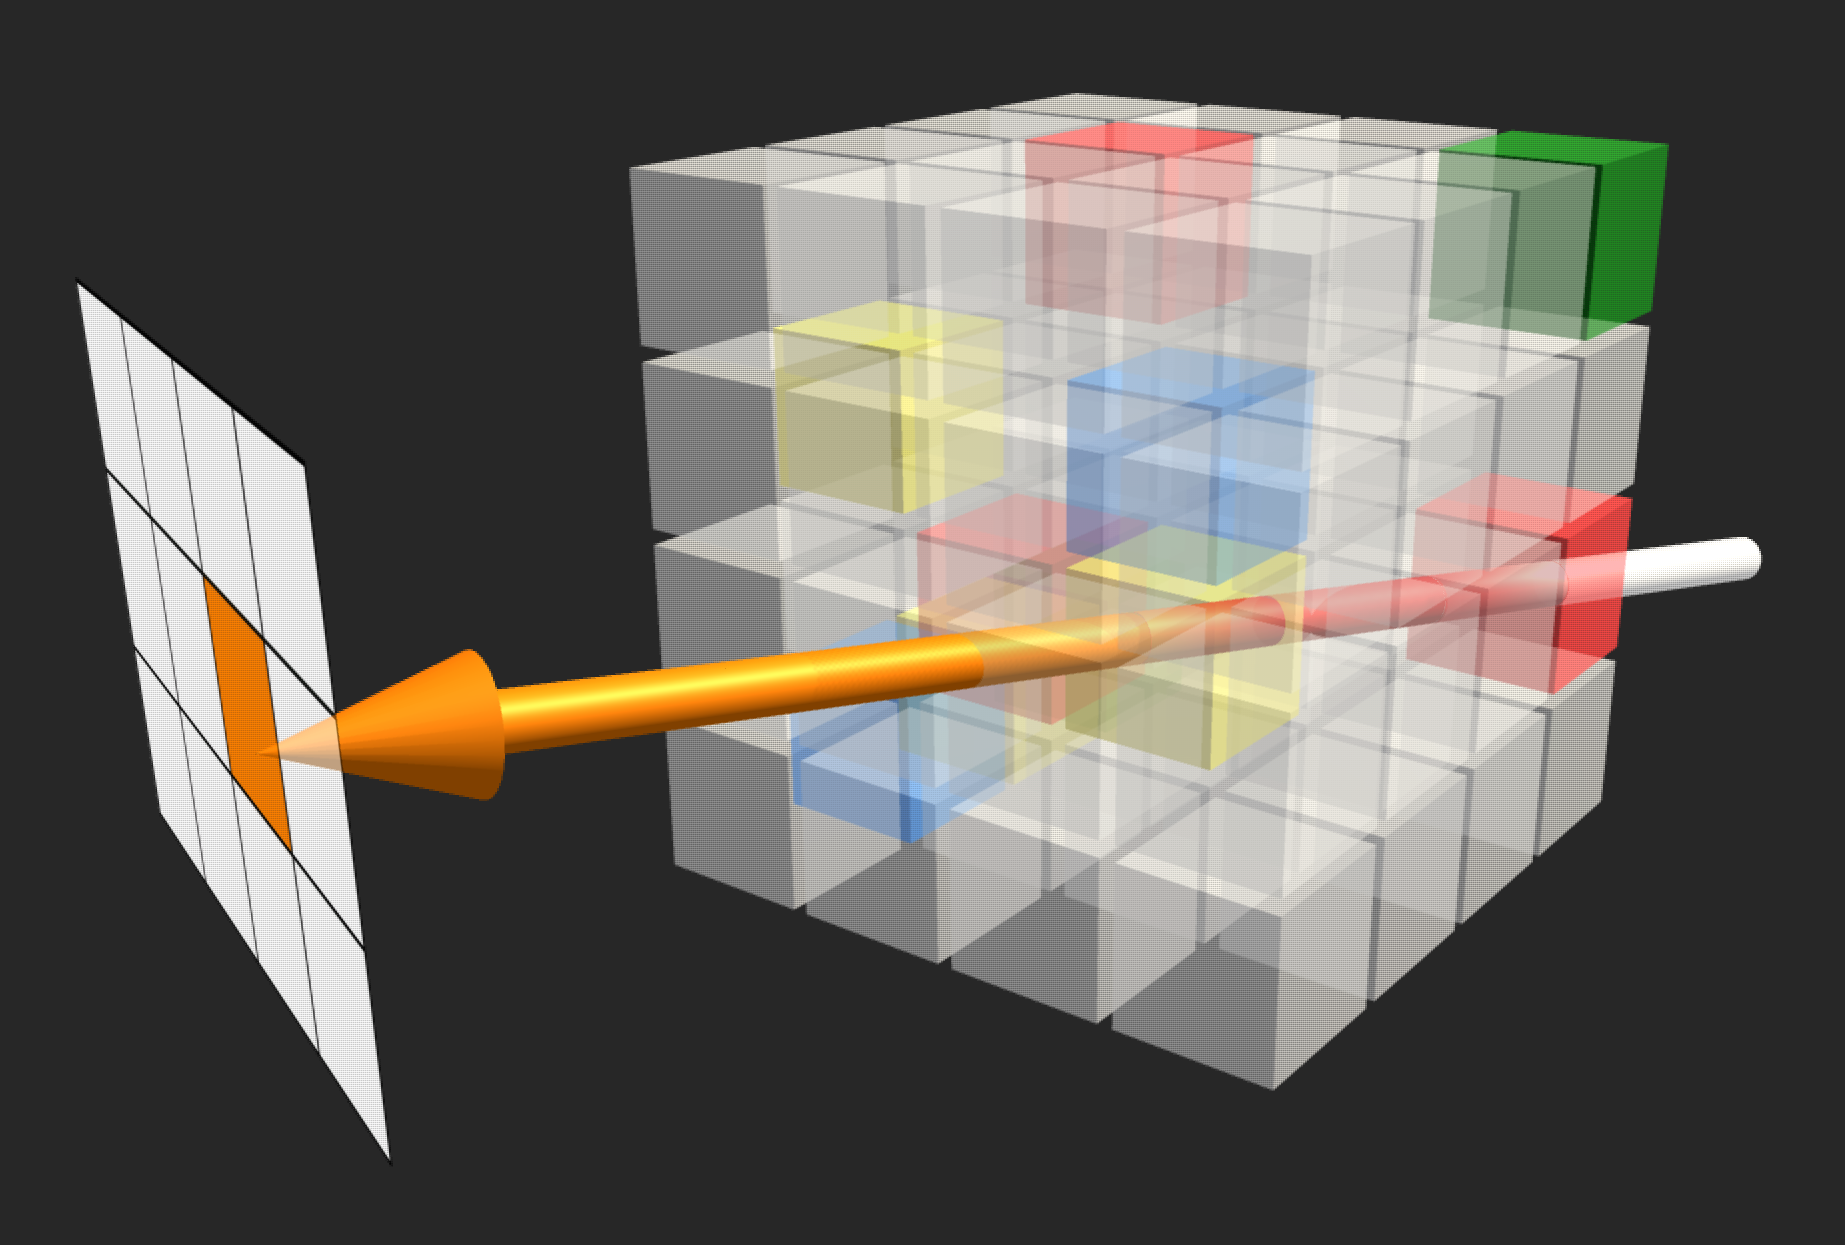
\includegraphics[width=1.0\textwidth]{ray-march-diagram}
\caption[FPBioimage: Raymarching facilitates volumetric rendering of 3D data]{In a traditional ray marching volumetric renderer, a colourless ray starts at the back of the volume, and picks up colour and transparency at each voxel it passes through. After its journey through the volume, it paints its accumulated colour to the screen pixel it lands on. }
\label{fig:raymarch-diagram}
\end{figure}

Volumetric rendering allows detail within the volume to be visualised~\cite{drebin1988volume}. 
By tuning the opacity of each voxel, details which would be invisible in a surface rendering can be seen in context, through the outer voxels of the model. 

The key drawback of volumetric rendering compared to geometric rendering is speed~\cite{dachille1998high}. 
In the simple volumetric renderer shown in Figure~\ref{fig:raymarch-diagram}, a ray is calculated for each pixel on the screen - 2$\times$\smaller[0.76]{10\textsuperscript{6}} pixels for a 1080p high definition display. 
If each ray takes \num{512} samples as it passes through the volume, each rendering of the volume requires over 1$\times$\smaller[0.76]{10\textsuperscript{6}} voxel calculations. 

When rendering a single volumetric image, or even a video which is first rendered then presented at a later time, this is not an issue: the rays can computed in parallel across a cluster of computers, and with some patience the images will build up. 
However, until recently displaying volumetric data at video rate in real time required specialised hardware optimised solely for volumetric rendering~\cite{ray2000resample}. 

The gaming industry has led to a rapid development of devices optimised for performing thousands of simple calculations in parallel. 
A single graphics processing unit (GPU) contains as many as 2560 individual processing cores~\cite{nvidia1080}, which can be used to calculate volumetric rays simultaneously. 
Combined with intelligent optimisations to the rendering algorithm, GPUs found in devices ranging from laboratory workstations to smartphones now enable real-time volumetric visualisation on personal computers. 

\subsection{WebGL enables volume rendering in a web browser}
Since the development of highly parallel GPUs, a handful of free and commercial programs have been released which provide volumetric rendering capabilities.
Popular software used in the microscope community includes ImageJ~\cite{schindelin2012fiji}, Icy~\cite{de2012icy}, and Imaris~\cite{imaris}; ITK-Snap~\cite{yushkevich2006user}, ParaView~\cite{ayachit2015paraview}, and ImageVis3D~\cite{imagevis3d2015interactive} are also used in the medical community for visualising patient data~\cite{madan2015creating}. 
These programs provide advanced offline volumetric rendering, and FPBioimage is not designed to replace them; instead, the key feature of FPBioimage is providing rendering on the web, to facilitate easy and interactive sharing of 3D data. 

The internet was originally designed to display static information, limiting web browsers' access to computational resources~\cite{leiner2009brief}.
However the relatively recent invention and widespread adoption of the Web Graphics Library (WebGL) now provides access to a GPU's processing power directly from the web browser~\cite{khronos2009webgl}. 
This means that three-dimensional effects on webpages can be rendered to the screen in real time.

In technical terms, WebGL exposes the \texttt{OpenGL ES 2.0} feature set \cite{khronos2009webgl}.
This is a shader-based application programming interface (API).
The API provides a limited number of simple functions which are optimised for running on GPUs in parallel. 

Figure~\ref{fig:caniusethis-webgl} shows that the support of WebGL is now widespread~\cite{caniuse}, available through HTML5 provided by all modern web browsers.

\begin{figure}[htb!]
\centering
\begin{subfigure}[b]{1.0\textwidth}
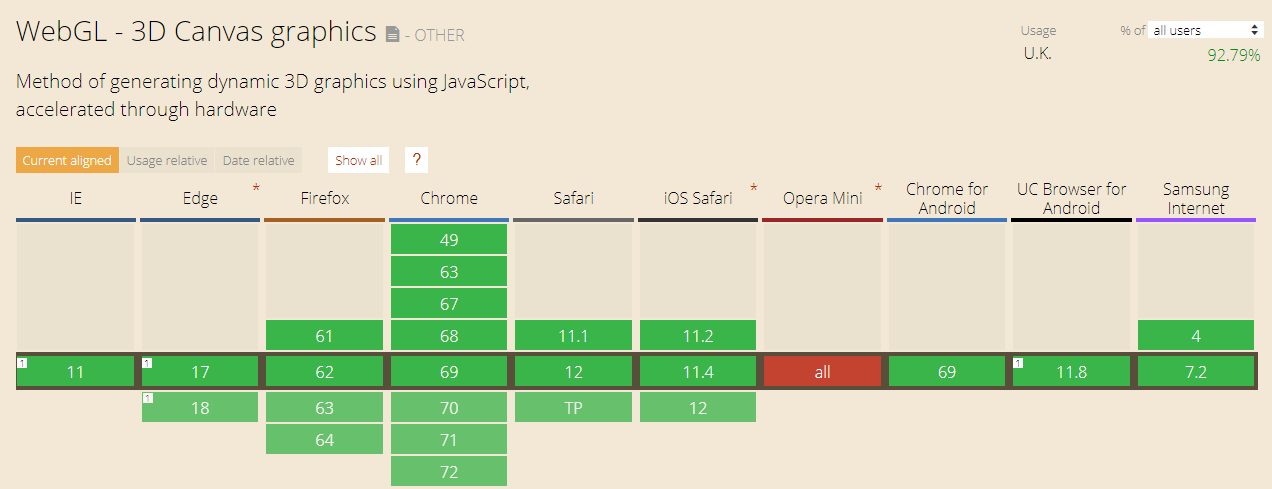
\includegraphics[width=1.0\textwidth]{caniusethis-webgl}
\caption{} \label{fig:caniusethis-webgl}
\end{subfigure}

~\newline
\begin{subfigure}[b]{1.0\textwidth}
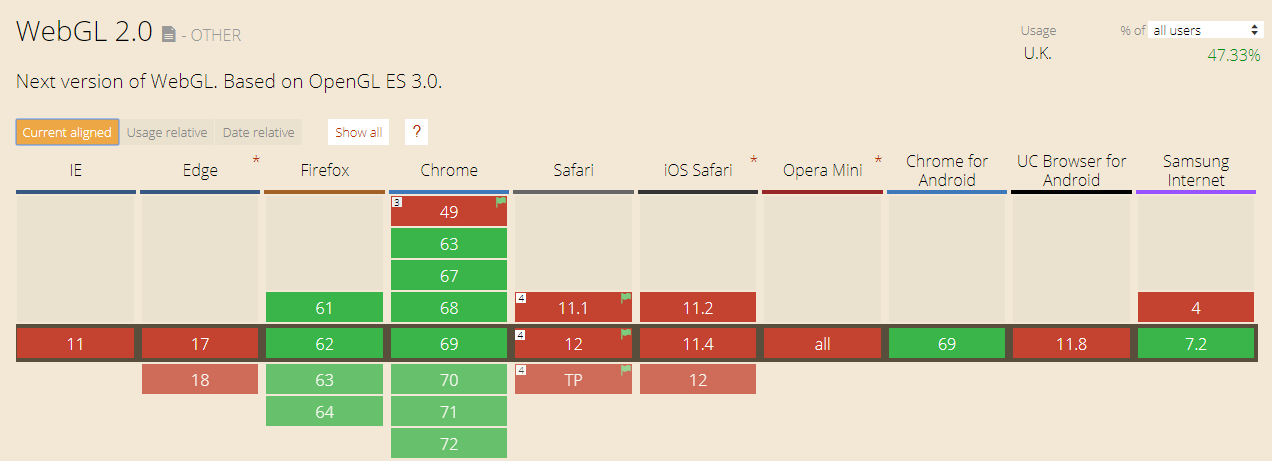
\includegraphics[width=1.0\textwidth]{caniusethis-webgl2}
\caption{} \label{fig:caniusethis-webgl2}
\end{subfigure}
\caption[FPBioimage: WebGL is supported by 92.79\% of users browsing the web]{Screenshots taken from \url{https://caniuse.com}\cite{caniuse}. (a) shows that FPBioimage, which is built with WebGL, is supported by the web browsers of 93\% of UK users. Although WebGL 2.0 makes 3D programming easier, (b) shows that support would drop to 47\% of users.  }
\label{fig:caniusethis}
\end{figure}

A more modern version, WebGL 2.0, exposes the \texttt{OpenGL ES 3.0} API, which makes programming for 3D much easier~\cite{webgl2}.
However, at the time FPBioimage was published, support for WebGL 2.0 was highly limited. 
Even at this time of writing, Figure~\ref{fig:caniusethis-webgl2} shows that WebGL 2.0 is only supported by third-party browsers, and cannot be used in Microsoft's Edge or Apple's Safari, limiting it to just \SI{47.33}{\percent} of UK web users~\cite{caniuse}.

To maintain maximum compatibility, volumetric rendering in FPBioimage is implemented entirely in WebGL 1.0.
Various strategies for overcoming this restriction are detailed in Section~\ref{sec:shader}.

\subsection{Aims for FPBioimage} 
The primary goal for FPBioimage was to create an easy-to-use web application for visualising volumetric data in a web browser; therefore a requirement was set that it must run without requiring any other plugins or downloads, in order that viewing data was a simple one-click process. 

After gathering user feedback, a full list of desired features was compiled. 

\begin{enumerate}
	\item Rendering options for more advanced users
	\item Ability to cut volumetric data open at arbitrary angles and positions (sometimes known as \textit{reslicing})
	\item Offer high resolution screenshots of the data
	\item Ability to save a particular view as a bookmark, and share that exact view with others
\end{enumerate}

For researchers sharing their own generated 3D data, more easy-to-use tools were proposed. 
These had to be compatible with popular image analysis programs, and facilitate fast sharing of volumetric data. 

From the first prototype FPBioimage was designed to be user-friendly. 
The program had to be intuitive so that a user could visualise their data without any training. 

\section{Method: software design} \label{sec:fpbSoftwareDesign}
This section describes, through the use of diagrams and code snippets, the method by which the volumetric visualisation software was developed.

The primary requirement of FPBioimage was that it must run in a web browser.
As mentioned in Section~\ref{sec:introvisual}, offline visualisation tools are already available, so the distinguishable feature of this software was the ability to share and publish volumetric data online.
For fast development and future-proof compatibility with multiple devices, I chose to develop the software in a game engine called Unity~\cite{unity}.
This gives access to an extensive library of functions for creating dynamic 3D scenes, as well as a language for executing code on the graphics card.
When the software is complete, Unity allows the designer to compile the `game' into compressed HTML/Javascript code to run in a web browser.

\subsection{The fragment shader calculates the colour of each screen pixel efficiently} \label{sec:shader}

\begin{lstfloat}
\begin{lstlisting}[language=C,caption={Fragment shader code for volumetric ray marching},label={snip:renderloop},frame=single]
// Fragment shader
float4 frag(frag_input i) : COLOR
{
	// Calculate eye ray (i) intersection with cube bounding box
	float3 boxMin = { -0.5, -0.5, -0.5 };
	float3 boxMax = {  0.5,  0.5,  0.5 };
	float tNear, tFar;
	bool hit = IntersectBox(i.ray_o, i.ray_d, boxMin, boxMax, tNear, tFar);
	if (!hit) discard;
	if (tNear < 0.0) tNear = 0.0;

	// Calculate intersection points
	float3 pNear = i.ray_o + i.ray_d*tNear;
	float3 pFar  = i.ray_o + i.ray_d*tFar;
	// convert to texture space
	pNear = pNear + 0.5;
	pFar  = pFar  + 0.5;

	// March along ray inside the cube, accumulating color
	float3 ray_pos = pNear;
	float3 ray_dir = pFar - pNear;
	float3 ray_step = normalize(ray_dir) / _Steps;

	float normalised_opacity = _Opacity * length(ray_step);
	float4 ray_col = 0;
	float mean_max_voxel = 0;

	for(int k = 0; k < MAX_STEPS; k++){
		if (k<_Steps){
			// Get current position
			ray_pos = pNear + k * ray_step;

			// Clip if behind clip plane or outside unit cube
			bool clipVoxel = dot(_ClipPlane, float4(ray_pos-0.5f, 1.0f)) > 0.0f
			 || !(ray_pos.x > 0.0f && ray_pos.y > 0.0f && ray_pos.z > 0.0f
			  && ray_pos.x < 1.0f && ray_pos.y < 1.0f && ray_pos.z < 1.0f);

			if (!clipVoxel && ray_col.a < 1.0f){
			  	// Get colour of the voxel we're passing through
		  		float4 voxel_col = sample2D(ray_pos);
			  	float mean_col = (voxel_col.r + voxel_col.g + voxel_col.b);

			  	if (_RenderMode == 0 && mean_col > _Threshold){
			  		// Max Intensity Projection
		  			if (mean_col > mean_max_voxel){
		  				ray_col = voxel_col;
		  				mean_max_voxel = (voxel_col.r + voxel_col.g + voxel_col.b);
		  			}

			  	} else if (_RenderMode == 1 && mean_col > _Threshold){
					// Volumetric ray marching with transparency
					voxel_col.a *= normalised_opacity;
					voxel_col.rgb *= voxel_col.a;
					ray_col += (1.0f-ray_col.a) * voxel_col;

				}
			}
		}
	}
	ray_col.rgb *= _Intensity;
    return ray_col;
}
\end{lstlisting}
\end{lstfloat}

FPBioimage uses a ray marching technique similar to that presented in Section~\ref{sec:volumerendering}.
The main ray marching loop implementing this is shown in lines Snippet~\ref{snip:renderloop}, based on NVIDIA's ``Render to 3D Textre'' guide~\cite{nvidia2008guide}.
This loop is part of the `fragment shader', which means it runs for every pixel rendered on the display.
It is therefore the most important loop in the whole program for efficiency, and any efforts to increase the speed at which this loop executes will be amplified by the number of pixels.
We will now examine the loop, and the efficiency modifications which have been made compared to traditional ray marching.

Lines 43 and 50 show that there are two different modes of rendering: a maximum intensity projection (\texttt{\char`_RenderMode == 0}) and the volumetric ray marching mode (\texttt{\char`_RenderMode == 1}) discussed in section \ref{sec:volumerendering}.
In the maximum intensity projection mode, the ray checks the mean colour of every voxel it passes through, and paints the colour of the voxel with the largest `mean color' to the screen pixel.
Note that mean colour is calculated as the sum of the red, green, and blue colour channels.
Strictly we should divide by $3$ to calculate the true mean colour value; however, this would mean 2 extra divisions for every loop iteration for every pixel on the screen; removing this step has no effect on the comparison, but gives an improvement in frames rendered per second. 

Before discussing the volumetric ray marching calculation, we should note that in this implementation the ray marches from the screen to the back of the cube - this is the opposite of traditional scheme shown in Figure~\ref{fig:raymarch-diagram}.
The reason for this is, of course, efficiency.
As a ray progresses from a pixel through the cube, it becomes more and more opaque, denoted by the alpha value of the colour \texttt{ray\char`_col.a}.
Once the alpha value reaches 1, any voxels further along the ray's path will not be visible, so there is no reason to look up their colour or add their contribution to the ray; line 50's second condition is that \texttt{ray\char`_col.a < 1.0f} to implement this behaviour.
Note that in most programming languages we would break out of the loop at this point, but WebGL 1.0 loops must have a constant number of iterations.

The requirement to have a constant number of iterations also explains the very first condition in the loop on line 29.
The variable \texttt{k\char`_Steps} sets the depth resolution of the volume.
We might expect the \texttt{for} loop to finish when \texttt{k < k\char`_Steps}, but this would set the depth resolution as a constant, removing the option to increase it for powerful machines or decrease it for mobile devices.
By looping for \texttt{MAX\char`_STEPS} iterations (which is currently set to 512, but could be increased as hardware improves in the future) but performing no calculations if the loop variables \texttt{k} is greater than \texttt{k\char`_STEPS}, we can set the depth resolution to any integer from 0 to \texttt{MAX\char`_STEPS} and gain a performance benefit for low resolutions.

There are two additional conditions which must be met for the volume renderer to add a voxel to the ray.
Firstly, shown in lines 34 to 38, the ray position must be within the unit cube and behind the clip plane.
The clip plane can be used to cut open the volumetric model at any angle and position, and is described in more detail in Section~\ref{sec:fpbResults}.
Secondly, the voxel's mean colour intensity must be above the value of \texttt{\char`_Threshold} to contribute to the ray, ensuring that dark voxels around the volume are not visible.

If all the aforementioned conditions are met, then the code in lines 49 - 51 performs the volumetric ray marching step - that is, the colour of the current voxel mixes onto the ray that is passing through it.
Firstly, the voxel's opacity is adjusted based on the input variable \texttt{\char`_Opacity}, which allows the volume to be rendered with transparency.
This new value of alpha is multiplied onto the voxel's colour so that more transparent voxels contribute less intensity to the ray.
Finally, the adjusted voxel is added to the ray, with its contribution weighted by the current transparency of the ray.

\subsection{A texture atlas scheme enables efficient loading of 3D data} \label{sec:fpbVolumeRendering}
To render volumetric images using the graphics card, the volumetric data must be loaded onto the graphics card in an appropriate format.
WebGL 2.0 provides a \texttt{sample3D} class, which is able to store 3D images and return a voxel colour at a requested 3D coordinate.
Unfortunately WebGL 1.0 does not have this functionality, and so an alternative scheme based on 2D textures has been devised.

The simplest way to picture volumetric imaging data is as a z-stack of 2D image slices.
One option to obtain a voxel colour at a given $xyz$-coordinate would be to store all 2D image slices, and look up the $xy$ value of the appropriate slice based on the $z$-coordinate.
This is conceptually simple, but inefficient to implement on a graphics card, as each slice must be sent to the graphics card individually, which is not only slow but adds a significant memory overhead to the graphics card loading process.
Instead, I devised a scheme where slices are stored on a large 2D texture atlas in a grid pattern.
Then, a voxel's $z$-coordinate corresponds to a specific slice on the grid, and the $xy$ components can be added to the bottom-left coordinates of that slice to obtain the $xyz$-coordinate voxel colour.

A restriction of WebGL 1.0 is a maximum texture size of 4096$\times$4096.
Using the atlas technique, this would support a maximum voxel resolution of 256$\times$256$\times$256.
This was found to be inadequate for most researchers' data, so a target of 512$\times$512$\times$512 was set.
In order to meet the requirements of WebGL 1.0, this requires 8 2D texture atlases of size 4096$\times$4096.

The 8 texture atlases are filled according to the pseudo-code shown in Snippet~\ref{snip:textureloading}.
The code uses a mixture of the modulo operator (\%) and division (/) to determine (a) which atlas to place each volume image slice in, and (b) the location in that image where the slice should be located.
Complementary code runs in the WebGL rendering code to read a particular voxel's colour given an $xyz$-coordinate.

\begin{lstfloat}
\begin{lstlisting}[language=java,caption={Java code for 3D texture atlas arrangement},label={snip:textureloading}]
int sliceWidth = volumeImage.width;
int sliceHeight = volumeImage.height;
int numSlices = volumeImage.depth; // Number of z-slices

int atlasWidth; int atlasHeight;
int numberOfAtlases = 8;

// Pad image size up to next power of 2
int paddedSliceWidth = ceil2(sliceWidth);
int paddedSliceHeight = ceil2(sliceHeight);

int xOffset = (int)Math.floor((paddedSliceWidth - sliceWidth)/2);
int yOffset = (int)Math.floor((paddedSliceHeight - sliceHeight)/2);

// Calculate the xy size of the atlases, making atlases as square as possible
int slicesPerAtlas = (int)Math.ceil((float)numSlices/(float)numberOfAtlases);
atlasWidth = ceil2(paddedSliceWidth);
atlasHeight = ceil2(paddedSliceHeight * slicesPerAtlas);
while((atlasHeight > 2*atlasWidth) && (atlasHeight > sliceHeight)) {
	atlasHeight /= 2;
	atlasWidth *= 2;
}

// Initialise an array of 8 black 2D textures to become atlases
Image[] atlasArray = new Image[numberOfAtlases];
for (int i=0; i<numberOfAtlases; i++){
	atlasArray[i] = new Image(atlasWidth, atlasHeight, black);
}

// Fill out atlases with image slices
int slicesPerRow = (int)Math.floor((float)atlasWidth/(float)paddedSliceWidth);
for (int i=0; i<numSlices; i++){
	int atlasNumber = (int)((float)i % (float)numberOfAtlases);
	int locationIndex = (int)Math.floor((float)i/(float)numberOfAtlases);

	// Get slice
	Image slice = volumeImage.getSlice(i);

	// Put slice into atlas at the correct position
	int xStartPixel = (int)((float)locationIndex % (float)slicesPerRow) * paddedSliceWidth + xOffset;
	int yStartPixel = (int)Math.floor((float)locationIndex / (float)slicesPerRow) * paddedSliceHeight + yOffset;

	// The following line should be uncommented for coordinate systems that start top-left
	//yStartPixel = atlasHeight - yStartPixel - paddedSliceHeight + 2*yOffset;

	copySubImageToAtlas(sliceTexture, atlasArray[atlasNumber], xStartPixel, yStartPixel);
}
\end{lstlisting}
\end{lstfloat}

% Should I add some paragraphs here about XY and Z resolution? Probably should.
%subsection{Rendering optimisation}
% XY resolution can be adjusted cleverly. 

% Z resolution can also be adjusted

% Interpolation

% Rendering paused when there is no user input. 

\subsection{Movement provides personal exploration of the data}
FPBioimage would not be a particularly exciting real-time volumetric renderer if the user only had one view of the data.
By utilising Unity library functions, implementing movement is a straightforward and resource-efficient process.

Firstly, as with all offline volumetric rendering programs, the 3D model can be rotated about its $x$-, $y$- and $z$-axes to view a different part of the data.
This is achieved in Unity by mapping the volume rendering shader described in Section~\ref{sec:shader} onto a cube.
The cube is then linked to both the arrow keys and to the mouse to provide intuitive manipulation of the volume, as shown in Snippet~\ref{snip:cuberotation}.
For data whose combination of $xyz$ resolution and $xyz$ voxel size describes a cuboid, the $xyz$ scale of the rendering cube can be adjusted to ensure distortion-free visualisation.

\begin{lstfloat}
\begin{lstlisting}[language={[Sharp]c}, label={snip:cuberotation}, caption={C\# code using built-in Unity functions to rotate the rendered volumetric data.}]
void FixedUpdate () {
	// This code is attached to the rendering cube, and called once per frame

	// Keyboard arrow control
	Vector3 vertRotAxis = transform.InverseTransformDirection(camera.TransformDirection(Vector3.right)).normalized;

	float horizontalRot = Input.GetAxis("H2");
	float verticalRot = Input.GetAxis("V2");

	transform.Rotate(vertRotAxis, verticalRot, Space.Self);
	transform.Rotate (Vector3.up, horizontalRot, Space.World);

	// Mouse click control
	if(Input.GetMouseButton(0)){
		// Rotate with the mouse
		Vector3 vertRotAxis = transform.InverseTransformDirection(camera.TransformDirection(Vector3.right)).normalized;

		float horizontalRot = Input.GetAxis("Mouse X");
		float verticalRot = Input.GetAxis("Mouse Y");

		transform.Rotate(vertRotAxis, verticalRot, Space.Self);
		transform.Rotate (Vector3.up, horizontalRot, Space.World);
	}
}
\end{lstlisting}
\end{lstfloat}

The `FP' in FPBioimage stands for `First Person,' and refers to the control the user has over the scene's camera.
Rather than just viewing the rotatable render cube from one perspective, as in common in offline volumetric renderers~\cite{schindelin2012fiji, de2012icy, imaris}, FPBioimage also allows the user to change the position and look-direction of the camera.
This is implemented as shown in Snippet~\ref{sec:cameramovement}.
The \texttt{H1} axis is mapped to the A and D keys, and the \texttt{Z1} axis to the W and S keys.
This, combined with the functionality of using the mouse to change the camera's look-direction, will make control of the camera very familiar to anyone who has played first person perspective computer games.
Moving the camera allows the user to create the type of dynamic fly-bys sometimes seen in publication videos in real time, providing a highly immersive visualisation of the data.

\begin{lstfloat}
\begin{lstlisting}[language={[Sharp]c}, label={sec:cameramovement}, caption={C\# code using built-in Unity functions for moving the camera in a first-person manner.}]
void FixedUpdate(){
	// Translation
	transform.position += Input.GetAxis ("V1") * Camera.main.transform.up * Time.deltaTime;
	transform.position += Input.GetAxis ("H1") * Camera.main.transform.right * Time.deltaTime;
	transform.position += Input.GetAxis ("Z1") * Camera.main.transform.forward * Time.deltaTime;
	transform.position += Input.GetAxis ("Mouse ScrollWheel") * Camera.main.transform.forward * Time.deltaTime;

	// Rotation
	if (!Input.GetMouseButton(1)) {
		// This is the 'first person' mouse mode
		rotationX += (Input.GetAxis ("Mouse X")) * mouseSpeed;
		rotationY += (Input.GetAxis ("Mouse Y")) * mouseSpeed;
		rotationY = ClampAngle (rotationY, minimumY, maximumY); // Stops camera doing backflips!

		Quaternion xQuaternion = Quaternion.AngleAxis (rotationX, Vector3.up);
		Quaternion yQuaternion = Quaternion.AngleAxis (rotationY, -Vector3.right);

		transform.localRotation = startRotation * xQuaternion * yQuaternion;
	}

	// Camera movement with mouse
	if (Input.GetMouseButton (1)) {
		transform.position -= Input.GetAxis("Mouse X") * Camera.main.transform.right * Time.deltaTime / Screen.width;
		transform.position -= Input.GetAxis("Mouse Y") * Camera.main.transform.up * Time.deltaTime / Screen.height;
	}
}
\end{lstlisting}
\end{lstfloat}

\subsection{Bookmarking is implemented with a state machine to share perspectives across the world}
FPBioimage implements a bookmarking function to save a particular view with an annotation.
The bookmarked view can then be shared with others as a web link, or restored on the same computer at a later time.

To implement the bookmark saving and restoring functionality requires several distinct actions, the order of which depends on the user's input.
An elegant method for reliably moving the user between these stages is a state machine.
The state machine controlling the bookmark saving and restoration procedures is shown in Figure~\ref{fig:bookmarking-state-machine}, and can be described as follows:
\begin{tabular}{>{\bfseries}l p{0.85\textwidth}}
State 0 & The default state, where all states eventually return to. Nothing regarding bookmarking is shown on the screen. Pressing `B' on the keyboard will start the bookmark creation process; pressing a number key will start the bookmark restoration process. Any other key does not change the state. \\
State 1 & The bookmarking textbox pops up requesting the user to enter a number key to save the new bookmark in that position. Pressing a number key will take the user to the next stage of bookmark creation; pressing `Escape' will close the textbox and return to the default state. \\
State 2 & The user can enter a text annotation into the text box. Pressing `Escape' will immediately close the textbox and return to the default state; pressing `Return' (also known as `Enter') will save the bookmark as described below and move to State 3. Note that an empty annotation is accepted. \\
State 3 & This state displays information or annotation text. If arriving from State 2, it will show a confirmation message; if arriving from State 4, it will show the annotation text saved alongside the bookmark being restored. \\
State 4 & This state simply checks that the volumetric model has loaded, to ensure no error is thrown if trying to restore a bookmark on an uninitialised volume. The state machine continues to wait in State 4 if the volume is loading, so any requested bookmark will be loaded immediately when the volume is ready. \\
\end{tabular}

\begin{figure}[htbp!]
\centering
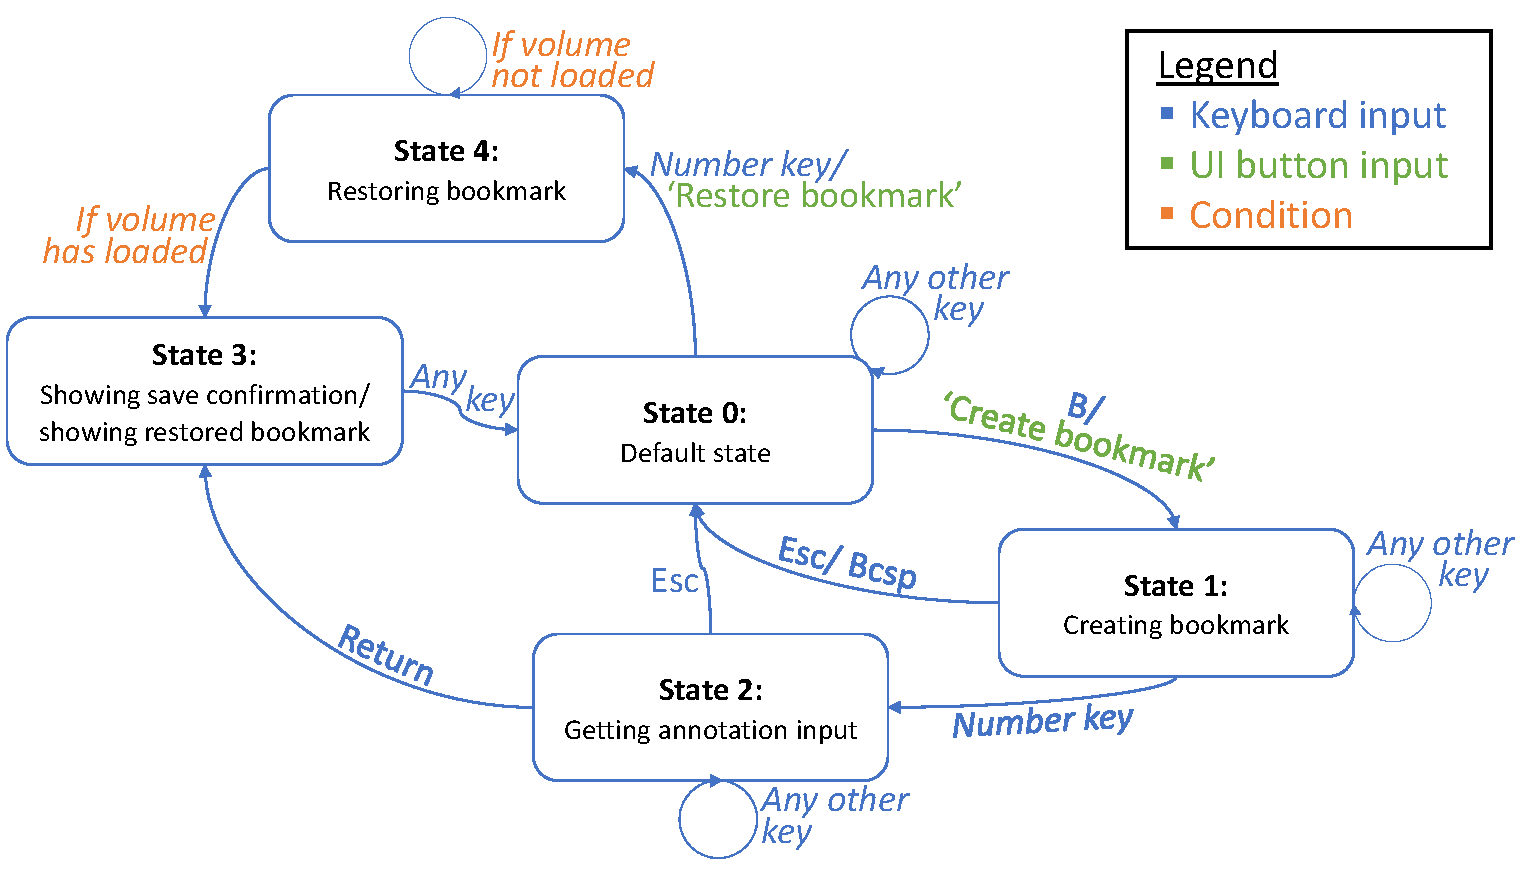
\includegraphics[width=1.0\textwidth]{bookmarking-state-machine}
\caption[FPBioimage: Bookmark creation and restoration is controlled by a state machine]{The state machine shown controls the creation and restoration of bookmarks. }
\label{fig:bookmarking-state-machine}
\end{figure}

Internally, the bookmarks are encoded as JavaScript Object Notation (JSON) strings, converted to a base-64 string, and then saved to the web browser's `Local Storage'.
Saving to Local Storage requires the C\# program to interface with the web browser through Javascript.
Unity provides the function \texttt{ExternalEval(string jscode)} to complete this task, where \texttt{jscode} is a string containing the JavaScript code to be executed.
Once the bookmark has been encoded, it is saved to the web browser as shown in lines 1 and 2 of Snippet~\ref{snip:savingbookmark}.
The bookmark is saved to Local Storage with a unique prefix followed by the bookmark's number, so that it can be restored at a later time.

\begin{lstfloat}
\begin{lstlisting}[language={[Sharp]c}, label={snip:savingbookmark}, caption={C\#-JavaScript interface code for interacting with the browser's local storage to save and share bookmarks.}]
string evalMe = "localStorage.setItem('fpb-" + variables.fpbJSON.uniqueName + "-bookmark" + bookmarkNumber + "', '" + bookmarkString64ToSave + "');";
Application.ExternalEval (evalMe);
evalMe = "history.replaceState(null, null, '?b=" + bookmarkString64ToSave + "');";
Application.ExternalEval (evalMe);
\end{lstlisting}
\end{lstfloat}

Lines 3 and 4 of Snippet~\ref{snip:savingbookmark} shows how the base-64 bookmark string is appended to the base url in the web browser using the JavaScript function \texttt{replaceState}.
The user can then simply copy the URL and send it to a friend or colleague to open on their own computer.
When the volume is being loaded, the bookmarking C\# script checks the URL of the webpage its running on, and if it finds a "\texttt{?b=}" in the URL string it will begin restoring the bookmark.
This puts the bookmarking state machine into State 4, ready to show the bookmark and annotation text as soon as the volumetric model has loaded.
In this way users can easily share specific views of the data across the globe.

\subsection{Screenshots can be captured at a higher resolution than the display}
FPBioimage provides the capture of high resolution screenshots, shown in Snippet~\ref{snip:screenshots}.

When the \texttt{takeScreenshot} function is called, a new \texttt{RenderTexture} is created to save the current view to.
The size of this can be set either by the current pixel size of the main camera or by user input.
In this way screenshots at a higher resolution than the current view can be created.
This is advantageous, as the user can view the volumetric data in a small window for fast performance, but then take a screenshot at a higher resolution for presentation and publication.

The new render texture is converted to a PNG-encoded byte stream, and then offered to the user as a download through the Javascript library \texttt{download.js}.
\texttt{download.js} provides a single function \texttt{download(data, strFileName, strMimeType)}, which is called from Unity using the C\#-JavaScript interface function \texttt{ExternalCall}.
This is shown in line 32 of Snippet~\ref{snip:screenshots}.

\begin{lstfloat}
\begin{lstlisting}[language={[Sharp]c}, label={snip:screenshots}, caption={C\# code for capturing a high-resolution screenshot and presenting it to the user as a download.}]
public void takeSreenshot(bool hiRes){
	if (hiRes) {
		bool wOK = int.TryParse (wRes.text, out ssWidth);
		bool hOK = int.TryParse (hRes.text, out ssHeight);

		if (!wOK || ssWidth < 1) {
			ssWidth = 1920;
		}
		if (!hOK || ssWidth < 1) {
			ssWidth = 1080;
		}
	} else {
		ssWidth = Camera.main.pixelWidth;
		ssWidth = Camera.main.pixelHeight;
	}

	// Create screenshot-sized render texture to render to
	RenderTexture rt = new RenderTexture(ssWidth, ssWidth, 24);
	mainCamera.targetTexture = rt;
	Texture2D snapShot = new Texture2D(ssWidth, ssWidth, TextureFormat.RGB24, false);
	mainCamera.Render();
	RenderTexture.active = rt;
	snapShot.ReadPixels(new Rect(0, 0, ssWidth, ssWidth), 0, 0);
	mainCamera.targetTexture = null;
	RenderTexture.active = null;
	Destroy(rt);

	// Encode snapshot to PNG byte stream
	byte[] bytes = snapShot.EncodeToPNG ();

	// Offer screenshot as download
	Application.ExternalCall ("download", "data:image/png;base64," + System.Convert.ToBase64String (bytes), "Screenshot " + System.DateTime.Now.ToString ("yyyy-MM-dd") + " at " + System.DateTime.Now.ToString ("HH.mm.ss") + ".png", "image/png");
}
\end{lstlisting}
\end{lstfloat}

\section{Results and discussion} \label{sec:fpbResults}
The FPBioimage software, designed in Unity as detailed in Section~\ref{sec:fpbSoftwareDesign}, was compiled into JavaScript to run in a web browser.
In this section, all screenshots and tests were performed in Google Chrome version 58 on the Windows 10 operating system.
However FPBioimage also runs flawlessly on any modern web browser, including Mozilla Firefox, Microsoft Edge, and Apple Safari, including mobile versions of these browsers.

\subsection{An intuitive interface requires no user training}
Great care has been taken to ensure FPBioimage is a user-friendly piece of software.
Many offline software packages already exist for rendering volumetric data; FPBioimage's unique selling point is that it runs in a web browser, to make sharing data with colleagues across the world a simple process.
For this reason it is important that a non-expert user can simply click on a link and use the software without any training.
At the same time as being immediately accessible to new users, the software also contains a number of advanced rendering options for those wishing to extract more information from the data.

\begin{figure}[htbp!]
\centering
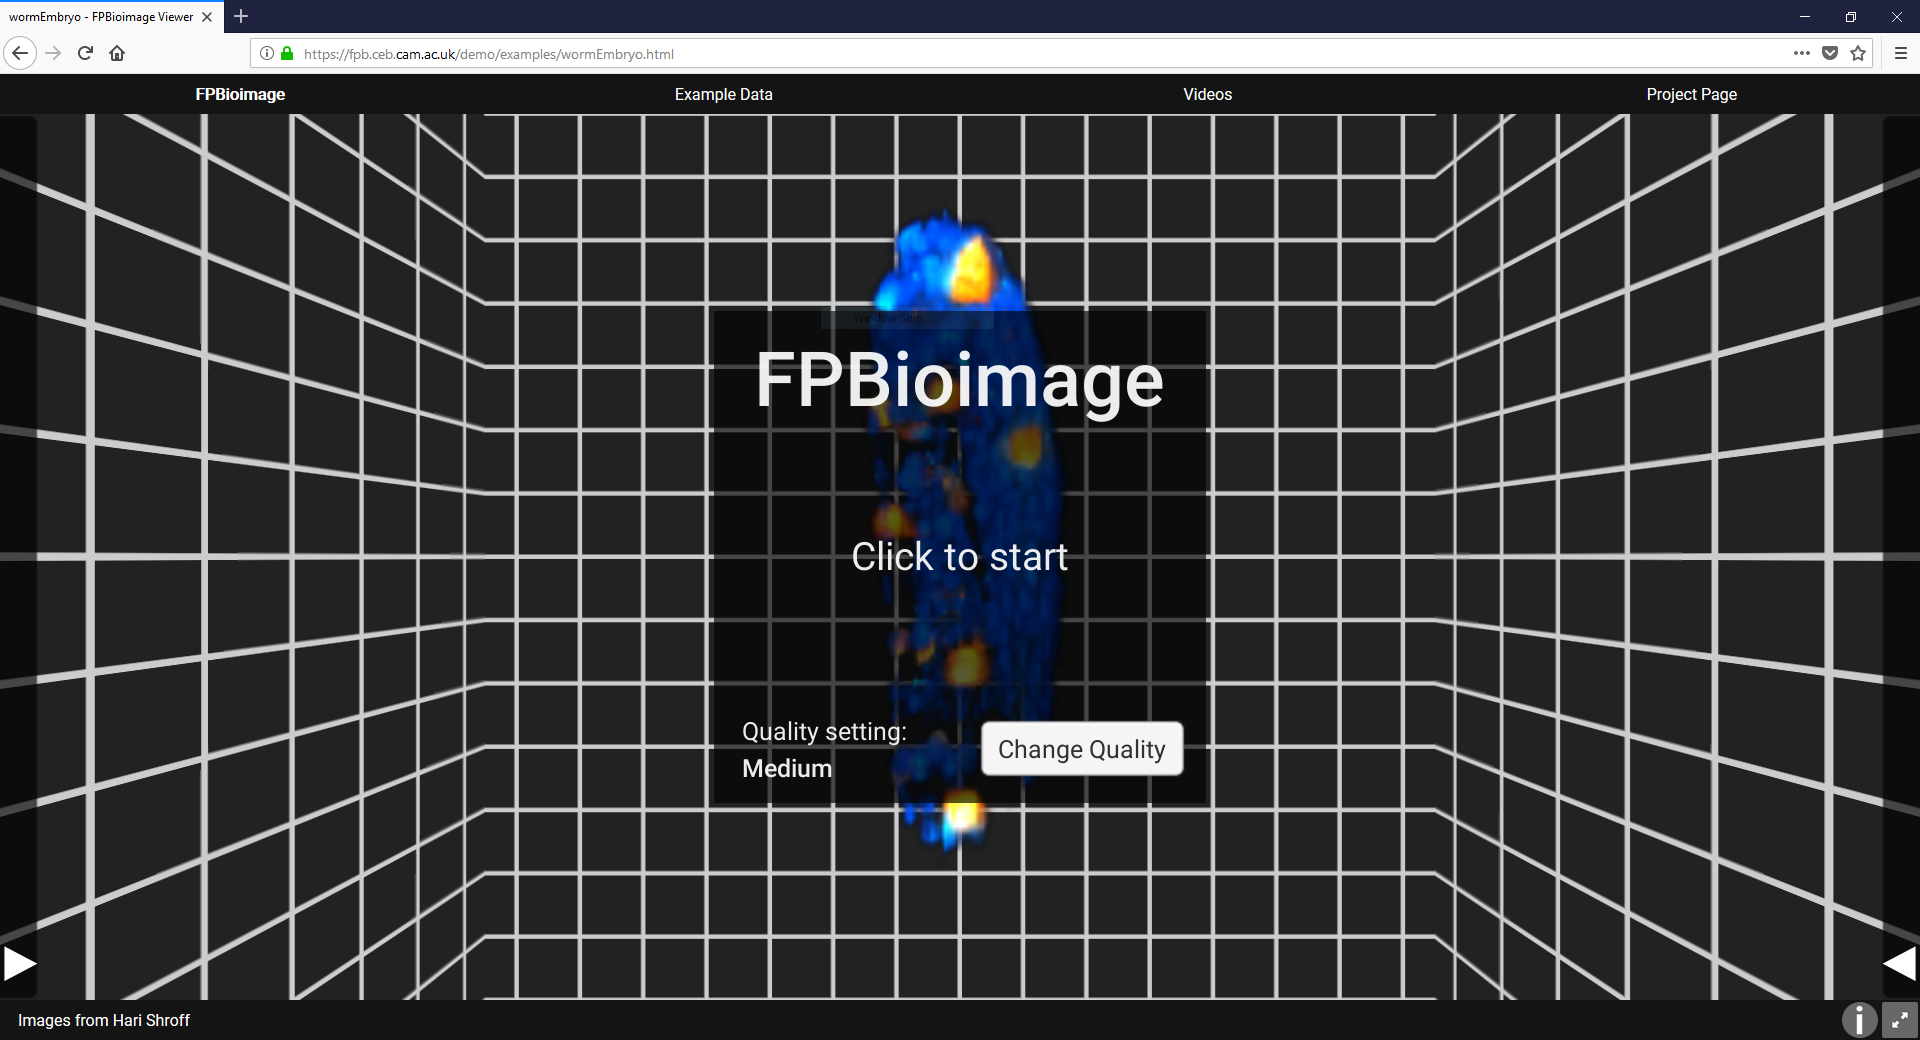
\includegraphics[width=1.0\textwidth]{fpb-start-screen}
\caption[FPBioimage: Users are presented with a simple interface which is intuitive to use]{When a user opens an FPBioimage webpage, the data will be downloaded and the user will be presented with the simple interface shown. The model can be interacted with intuitively by clicking and dragging with the mouse, or finger on a touchscreen. The data shows a C. Elegans embryo captured by single plane illumination microscopy (SPIM), provided by Hari Shroff~\cite{kumar2014dual}. }
\label{fig:FPBhome}
\end{figure}

When opening up a web link with FPBioimage on the page, the user is presented with the view shown in Figure~\ref{fig:FPBhome}.
Interacting with the volumetric model is responsive and intuitive.
Using the mouse, the user can rotate the volume by clicking and dragging, or on a touch screen by dragging with their finger.
Alternatively the arrow keys can be used on a keyboard.
Pinching on a touch screen, or using the scroll wheel on a mouse, zooms in and out of the model.
This creates a natural interaction with the data that requires no additional instruction.

\begin{figure}[htbp!]
\centering
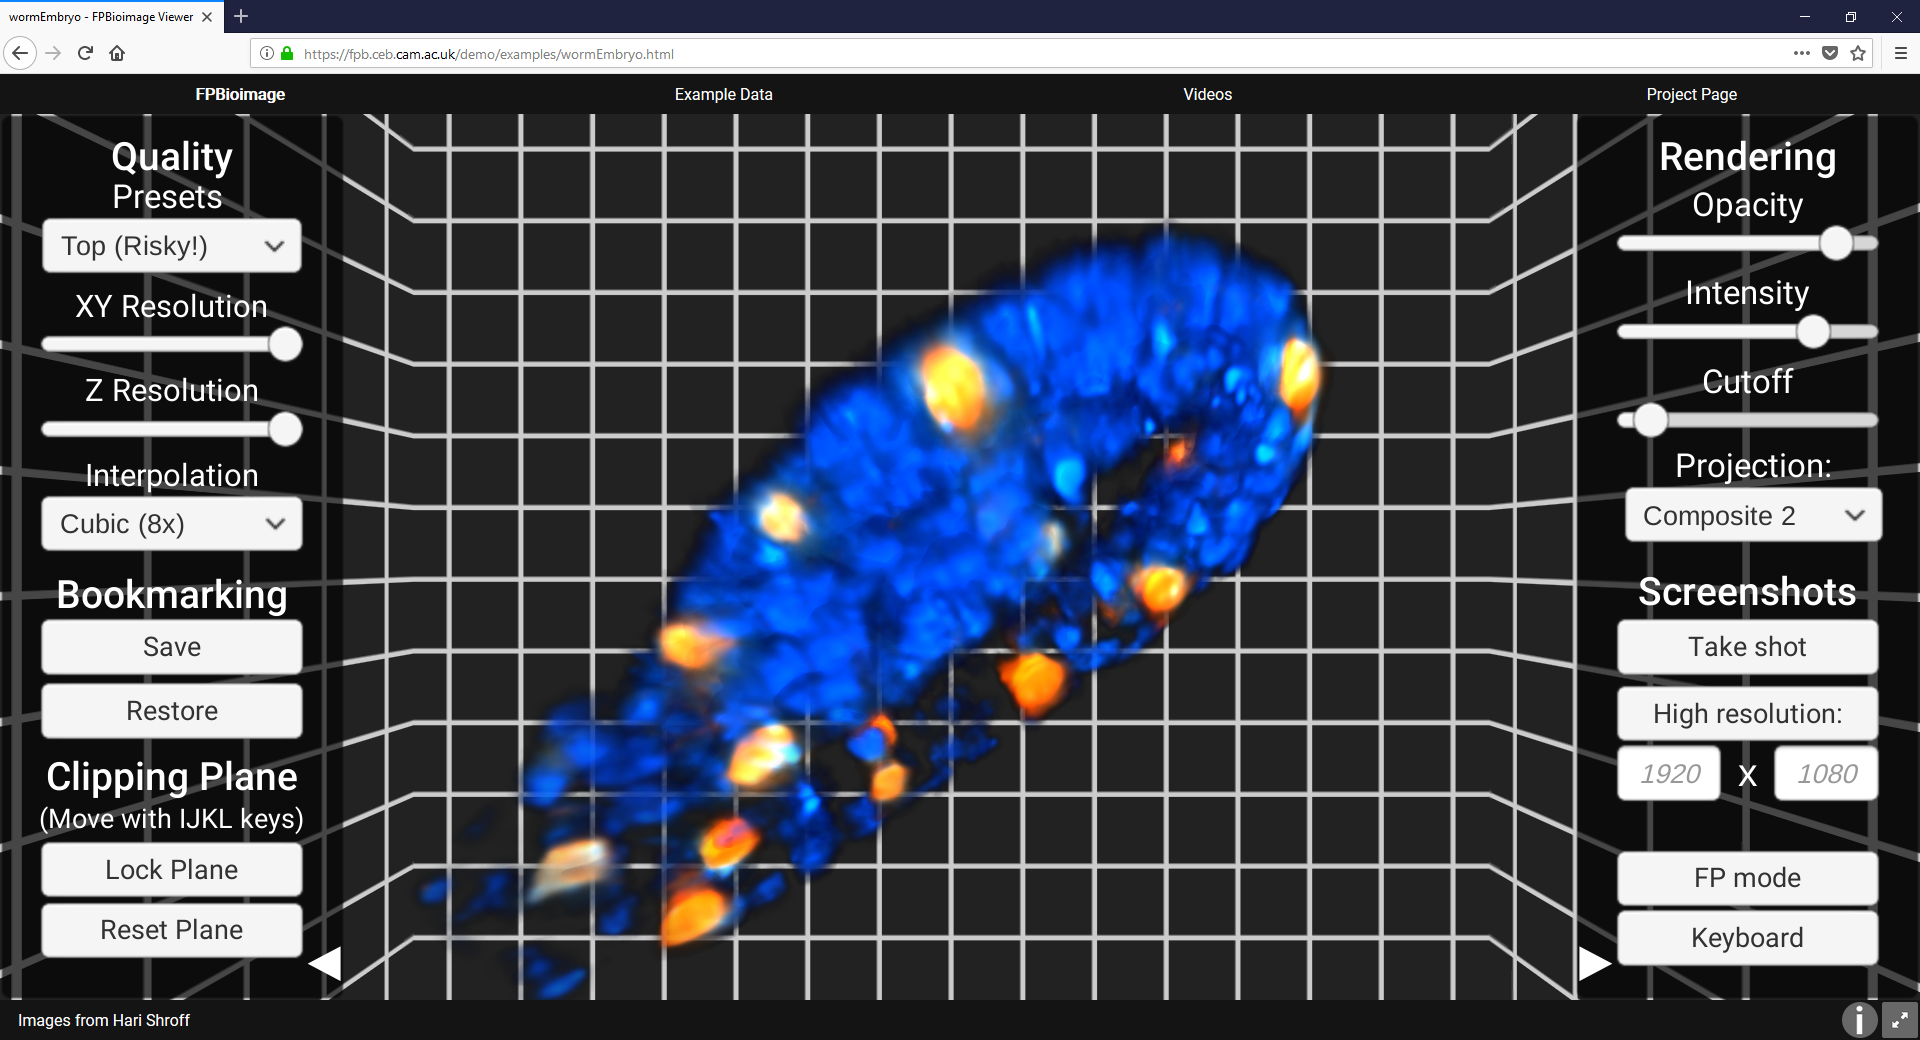
\includegraphics[width=1.0\textwidth]{fpb-side-panels}
\caption[FPBioimage: Side panels provide more advanced rendering options]{Clicking on the side panel arrows slides in advanced rendering options, clipping plane options, quality options, and bookmark and sharing options. Data from~\cite{kumar2014dual}. } % 
\label{fig:FPBpanels}
\end{figure}

To access more advanced rendering features, Figure~\ref{fig:FPBpanels} shows a panel on the right-hand side of the screen which slides in.
The user is presented with 3 rendering parameters: \textui{Opacity}, \textui{Intensity}, and \textui{Cutoff}.
Matching these parameters up to the volume rendering code described in Section~\ref{sec:fpbVolumeRendering}, it is easy to see how each parameter modifies the presentation of the data.

\begin{sidewaysfigure}[p]
\centering
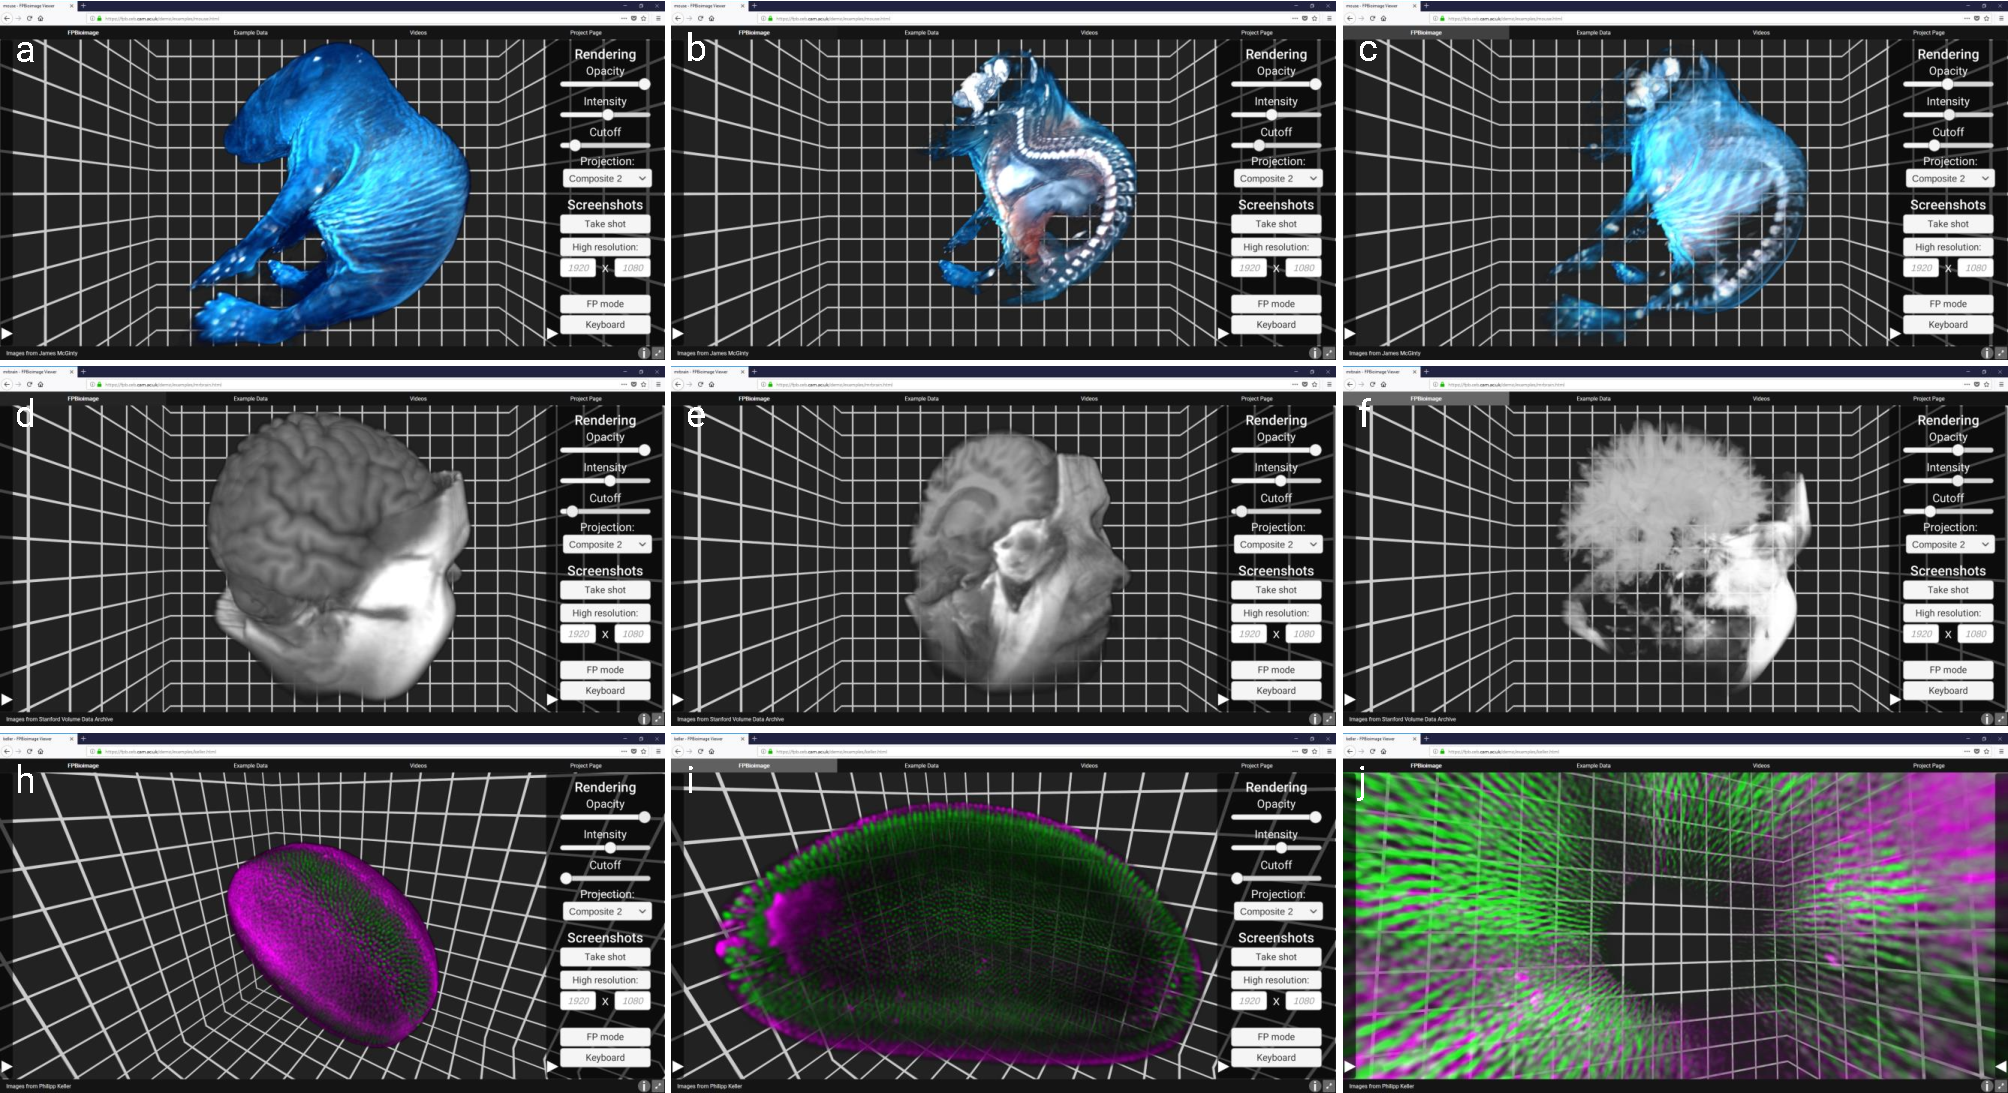
\includegraphics[width=\textwidth]{fpb-sliders-examples} % If possible separate caption onto new page? 
\caption[FPBioimage: Advanced rendering features provide unique views of volumetric data]{(a–c): Four-colour OPT data of a mouse embryo. (d–f): MRI data of a human head. (g–i): two-colour light-sheet microscopy data of a drosophila embryo. FPBioimage's built-in transparency feature has been used to render (c) and (f), revealing data within the volume; the cutting tool has been used for (c), (f), (h) and (i), removing outer voxels from the data; and h shows a bookmark in creation, which can be shared with other users. Reproduced from \cite{fantham2017new}. Raw data provided by: (a–c), J. McGinty~\cite{sharpe2002optical}; (d–f), Stanford Volume Data Archive~\cite{levoy1988volume}; (g–i), P. Keller~\cite{chhetri2015whole}. }
\label{fig:fpbRendering}
\end{sidewaysfigure}

Lowering the \textui{Opacity} value means that each voxel contributes less alpha to the ray marching through it; consequently, the volumetric data becomes more transparent.
This makes features inside the model visible through the outer voxels, as shown in Figure~\ref{fig:fpbRendering}.
Combined with rotating the volume, this facilitates visualisation of how different structures are arranged in 3D space, providing answers that are not possible to obtain in any other way.

The \textui{Intensity} value acts globally on the data at the end of the ray marching process.
This simply increases or decreases the overall brightness of the model, to reveal contrast either at the bright end or the dark end of voxel values. % should I actually make this change the response curve??

The \textui{Cutoff} slider sets the value below which voxels are not rendered.
Most microscopy images, as well as images from other modalities such as MRI, use black voxels around the imaging data to represent a lack of light or objects.
Settings a small positive value for \textui{Cutoff} ensures that the volume does not appear as a black box when \textui{Opacity} is set high.
Larger values for \textui{Cutoff} can also be used to highlight bright objects which lie within the volume.

The next element in the right-hand UI tab is the \textui{Projection} dropdown menu.
As described in Section~\ref{sec:fpbSoftwareDesign}, FPBioimage provides several volumetric visualisation rendering pipelines.
These include \textui{Max. Intensity}, which renders a maximum intensity projection from any angle; and \textui{Composite}, which performs volumetric ray tracing with support for transparency.
Furthermore the \textui{Iso-surface} projection reveals only voxels within a certain percentage of the \textui{Cutoff} voxel value.
Screenshots of the various \textui{Projection} methods rendering a mouse embryo head are shown in Figure~\ref{fig:fpbProjections}.

\begin{sidewaysfigure}[p]
\centering
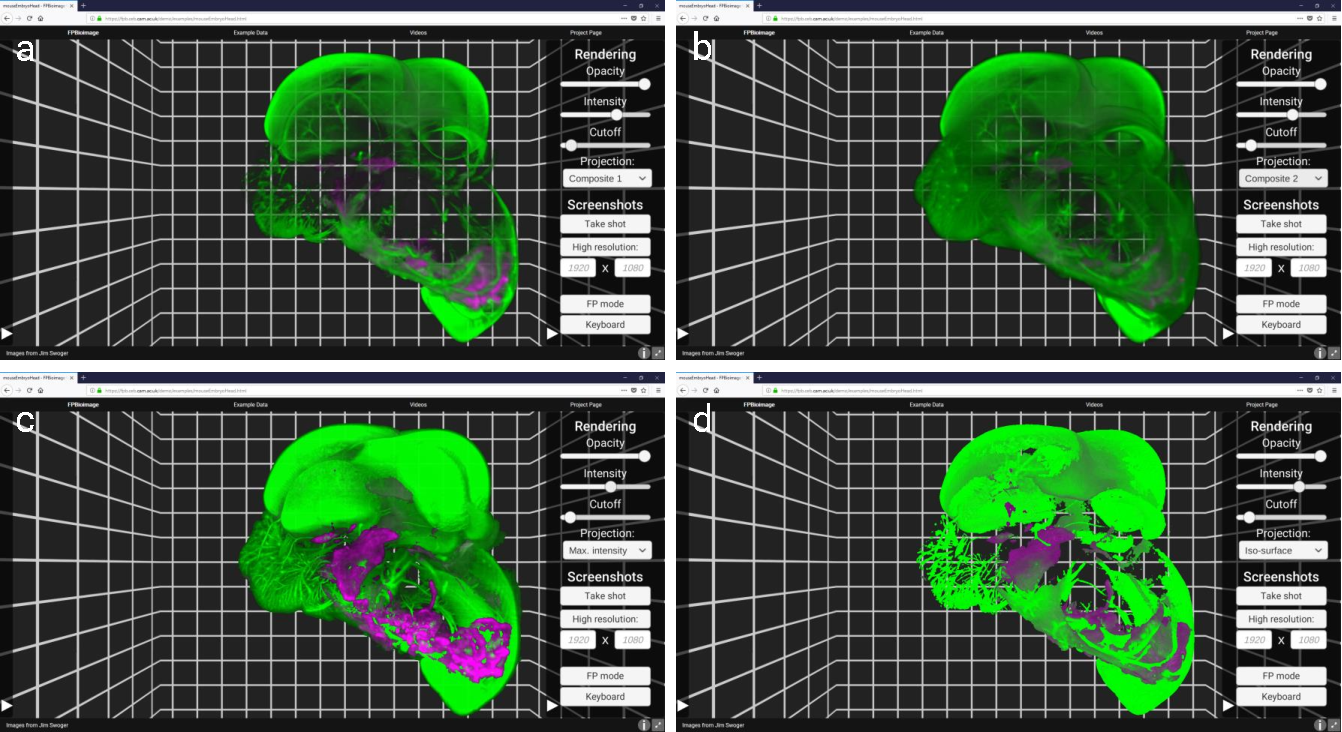
\includegraphics[width=\textwidth]{fpb-projections}
\caption[FPBioimage: Four projection methods highlight different details in volumetric data]{First Person Bioimage offers 4 different types of volumetric projection. (a) shows a maximum intensity projection, (b) a volumetric ray marching projection, (c) a variation on the volumetric ray marching projection, with alpha calculated from RGB voxel values, and (d) an iso-surface projection. Data is of a mouse embryo head captured with `OPTiSPIM', provided by Jim Swoger~\cite{mayer2014optispim}. }
\label{fig:fpbProjections}
\end{sidewaysfigure}

Further down the right-hand UI tab are two UI buttons for capturing screenshots.
The first, \textui{Take shot}, captures a screenshot at the current resolution of the drawing canvas.
Perhaps more usefully, the \textui{High resolution} screenshot button captures a screenshot at the resolution defined in the two text boxes below.
This allows the user to capture screenshots at a higher resolution than their display, in case high resolution images are required for presentation or publication.
The advantage of this is exemplified in Figure~\ref{fig:fpbScreenshots}.

\begin{figure}[htbp!]
\centering
\begin{subfigure}[b]{1.0\textwidth}
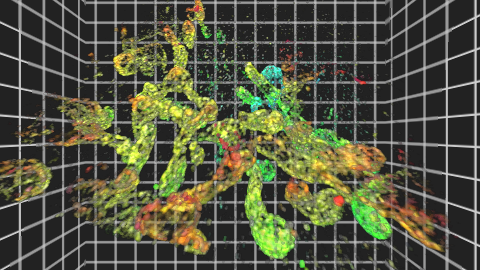
\includegraphics[width=1.0\textwidth]{fpb-screenshot-low}
\caption{}
\end{subfigure}

~\newline
\begin{subfigure}[b]{1.0\textwidth}
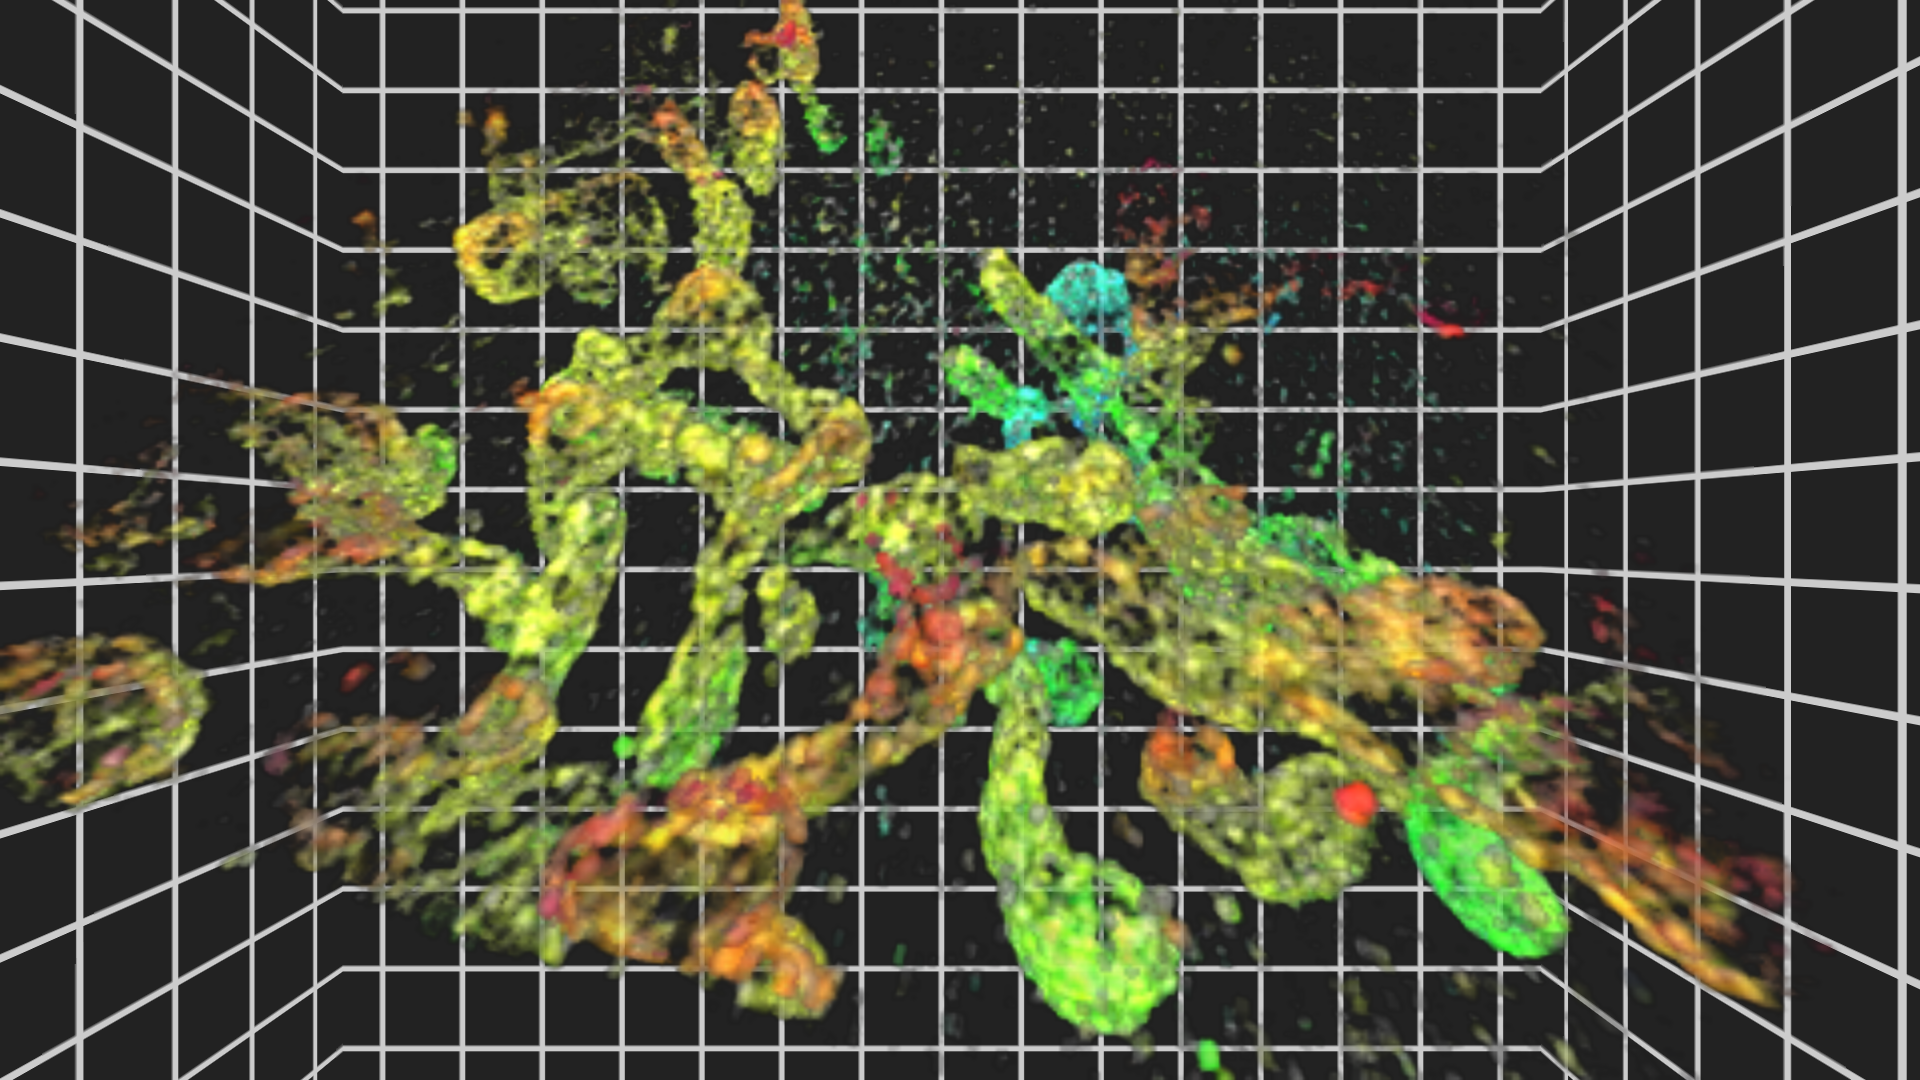
\includegraphics[width=1.0\textwidth]{fpb-screenshot-high}
\caption{}
\end{subfigure}
\caption[FPBioimage: Screenshots allow views to be captured at a higher resolution than the user's display]{High resolution screenshots can be created even on a small display. (a) shows a screenshot at the native 768x1024 display resolution; (b) shows a 1080p screenshot of the same view, created using the \textui{High resolution} button. Images are of mitochondria captured with a whole-cell 4Pi single-molecule switching nanoscopy (W-4PiSMSN) microscope, provided by Joerg Bewersdorf~\cite{huang2016ultra}. }
\label{fig:fpbScreenshots}
\end{figure}

The final two buttons in the right-hand UI tab are toggle buttons, labelled \textui{FP mode} and \textui{Keyboard}.
\textui{FP mode} toggles on the First Person mouse control that gives FPBioimage its full name.
In this mode the user can use the mouse to look around, in a way that is familiar to anyone who has played a first-person perspective game.
This can provide dramatic and immersive flights through the data controlled by the user, revealing much more information than can be provided on a pre-recorded video.
First Person control is shown in Supplementary Video 1 included with this document.

At all times (except when creating a bookmark), the user can use the WASD keys to move around, as shown when the \textui{Keyboard} button is active.
Pressing the \textui{Keyboard} button brings up a full list of controls, presented in Figure~\ref{fig:fpbMenu}.
Every rendering option is available through a keyboard shortcut, for complete mouse-free operation.

\begin{figure}[tbp!]
\centering
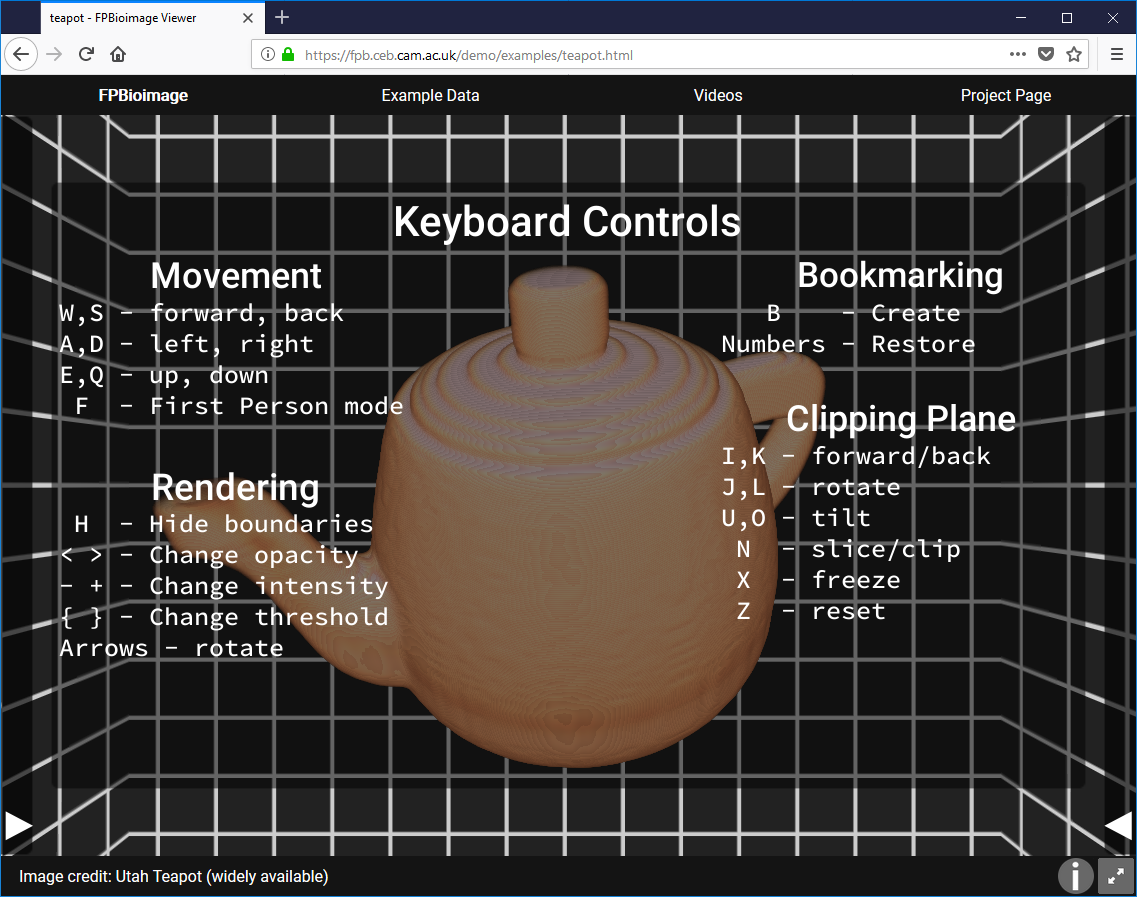
\includegraphics[width=1.0\textwidth]{fpb-menu}
\caption[FPBioimage: Keyboard controls allow FPBioimage to be used without a mouse]{All rendering options in FPBioimage can be controlled by the keyboard, for mouse-free operation. The teapot in the background is the widely available Utah teapot created by Martin Newell~\cite{torrence2006martin}. }
\label{fig:fpbMenu}
\end{figure}

The left-hand UI tab reveals yet more parameters which can be controlled by a more advanced user.

The first of these is \textui{Quality}.
Volume rendering in real time is a graphics-intensive operation which has only recently become possible, and there is a clear trade off between quality and performance on most computers or mobile devices.
A dropdown list shows a selection of preset options with suggestions of the type of device they are suitable for.
For more advanced users, the individual quality settings \textui{XY Resolution}, \textui{Z Resolution}, and \textui{Interpolation} can be adjusted independently.
The \textui{Quality} settings are saved to the web browser's Local Storage upon modification and are automatically restored on the user's next visit to an FPBioimage webpage.
The performance-quality trade-off is discussed in more detail in Section~\ref{sec:fpbPerformance}.

The bookmarking functionality can be accessed from the UI using the \textui{Save} and \textui{Restore} buttons.
This begins the state-machine process shown in Figure~\ref{fig:bookmarking-state-machine}.
Creation of a bookmark is shown in Figure~\ref{fig:fpbBookmarkCreation}.
When a bookmark is created or restored, the URL in the browser bar changes to encode the bookmark as a web link.
This link can then be shared with other users, by email, text, or on social media, who will see exactly the same view when FPBioimage loads.
This is demonstrated in Figure~\ref{fig:fpbBookmarkRecieved}, where the shared bookmark is opened on another computer, with a different browser and operating system.

\begin{figure}[htbp!]
\centering
\centering
\begin{subfigure}[b]{1.0\textwidth}
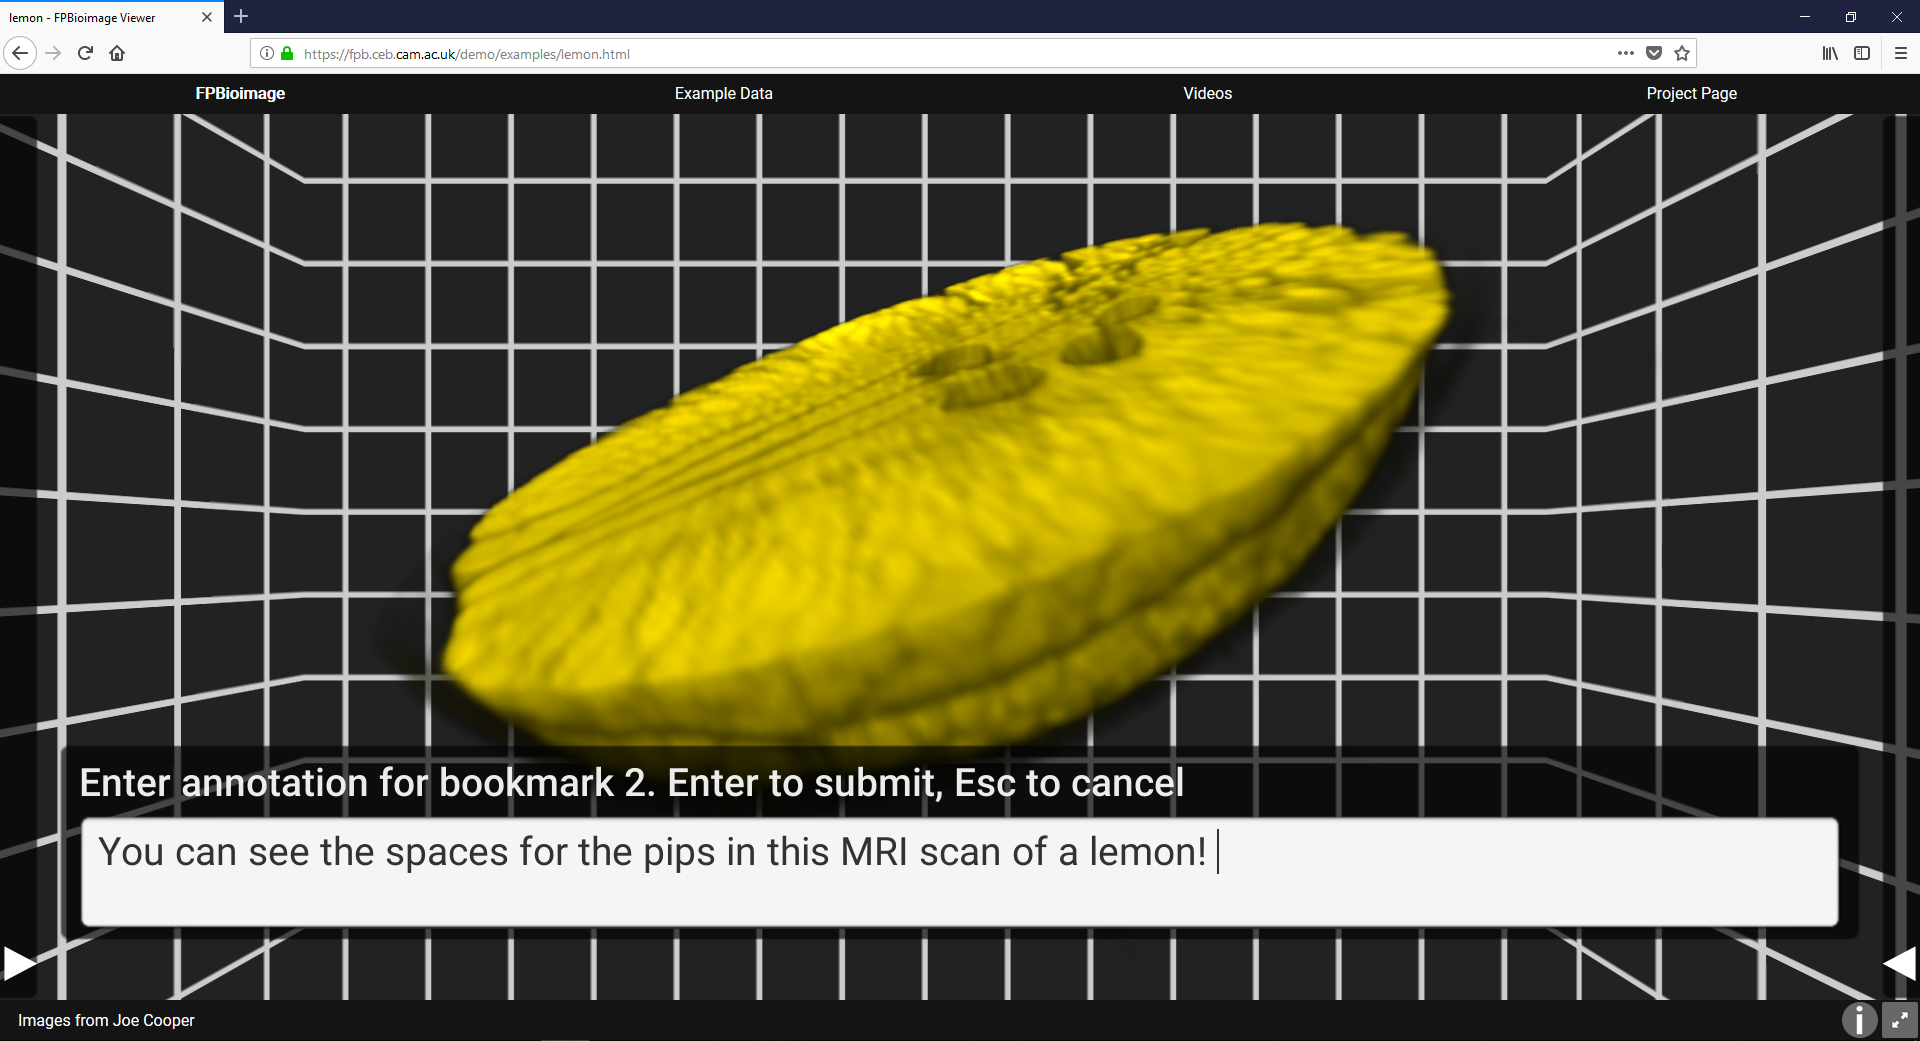
\includegraphics[width=1.0\textwidth]{fpb-bookmarks}
\caption{} \label{fig:fpbBookmarkCreation}
\end{subfigure}

~\newline
\begin{subfigure}[b]{1.0\textwidth}
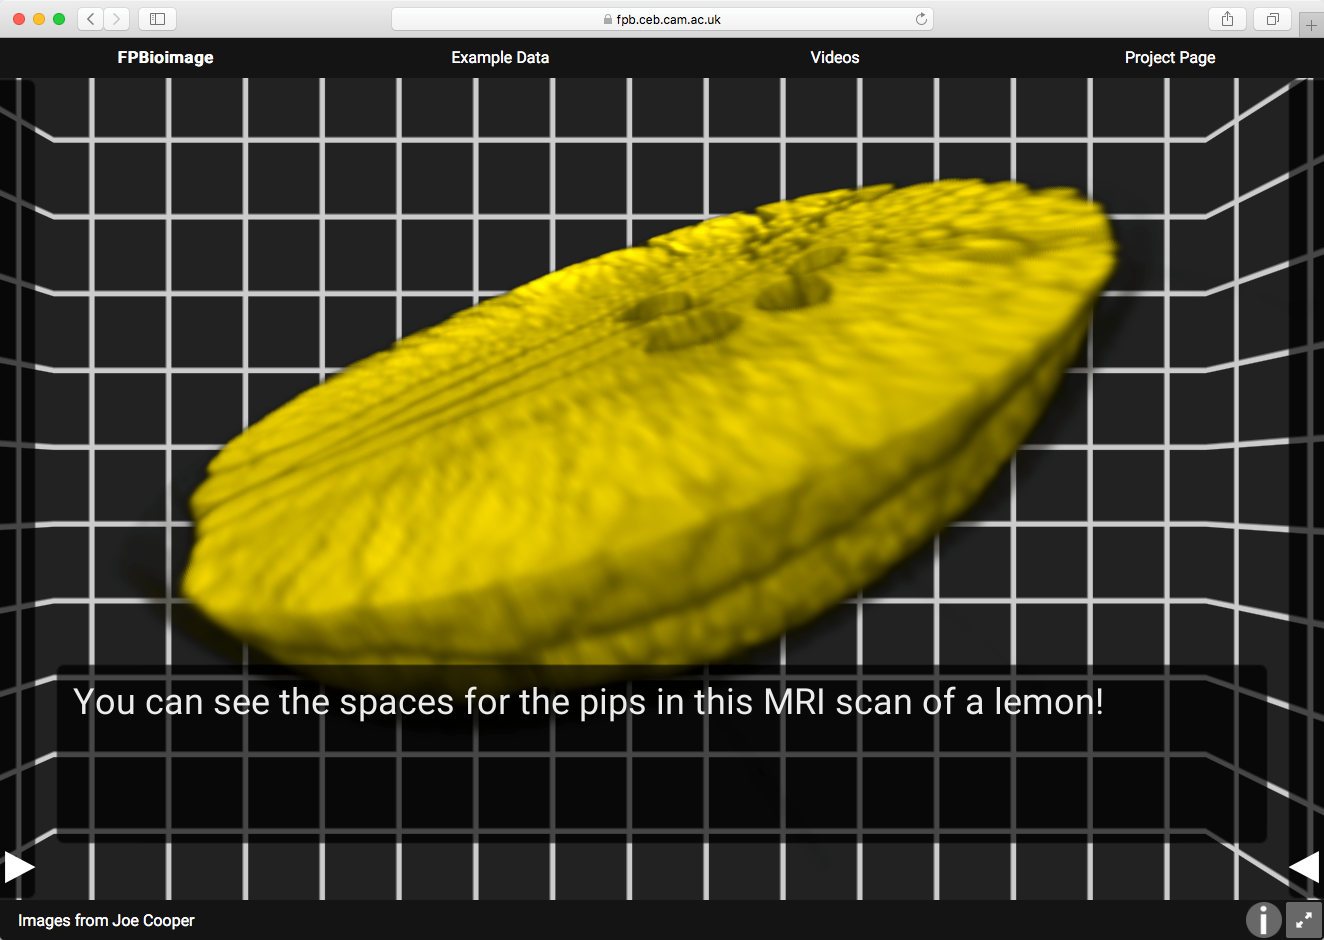
\includegraphics[width=1.0\textwidth]{fpb-bookmark-sharing}
\caption{} \label{fig:fpbBookmarkRecieved}
\end{subfigure}
\caption[FPBioimage: Bookmarks can be shared as a URL for another user to open]{(a) shows creation of a bookmark, with an annotation, in the Firefox web browser running on Windows 10. The bookmark can be restored on the same computer, or shared as a URL to another user. (b) shows the same bookmarked view in Apple Safari running on macOS 10.13 High Sierra. The MRI scan of a lemon was provided by Joe Cooper. }
\label{fig:fpbBookmarks}
\end{figure}

Finally, at the bottom of the left-hand UI tab are the UI buttons for the clipping plane.
Mentioned briefly in Section~\ref{sec:fpbVolumeRendering}, the clipping plane prevents voxels that are behind it from being rendered, revealing voxels inside the volumetric data that are otherwise obscured.
The clipping plane's location is controlled with the IJKL keys, where I and K are used to move the clipping plane forward and back, and J and L rotate is around to cut the data at an arbitrary angle.
Once an interesting cut has been made, the clipping plane can be locked in place with respect to the model by pressing the \textui{Lock Plane} button.
With the clipping plane locked, the user can move the camera or the model to view the cut volumetric data from a different angle.
Use of the clipping plane can therefore provide insightful perspectives of the volumetric data that are not possible to obtain with any other method, as shown in Figures~\ref{fig:fpbRendering}b, e, h, and i.

\subsection{Measuring performance reveals compatibility with consumer-grade computers} \label{sec:fpbPerformance}
Until recently, volume rendering was not possible in real time, and would be calculated for a specific camera perspective in advance of presentation to render either a single image or video.
In 2000, Ray and Silver produced the Race II Engine, designed with dedicated hardware to render [512$\times$512$\times$512] volumetric images in real time.
This was achieved by realising the volume rendering algorithm described in Section~\ref{sec:volumerendering} with physical devices, with hundreds of calculations running in parallel to compute all rays at once~\cite{ray2000race}.
Today, top-end graphics cards are able to perform the same calculations in real time on a Graphics Processing Unit (GPU), a highly parallelised device optimised for computing lighting models~\cite{lindholm2008nvidia}.

A primary aim of FPBioimage was that it should be user-friendly, with a particular focus on ease-of-use for non-expert users viewing data.
It was therefore expected that a majority of users would not have access to expensive, high-performance graphics cards required for rendering volumetric data in real time at full resolution.
Furthermore FPBioimage was designed so that it could be run on any device - Statista statistics show that over 40\% of web traffic in August 2018 was from mobile browsers~\cite{statistica2018mobile}.
In order to support the full range of users, it was important to devise a scheme where the user could reduce the quality of the volume rendering in exchange for an increase in performance.

In the computer games industry, ``performance'' essentially means how many frames are rendered to the screen per second - assuming the graphics card is working at full capacity.
If the graphics rendering does not require the full capacity of the graphics card, performance can be measured as the percentage of the graphics card's compute capabilities in use.
In the tests presented in this chapter, performance is given in both frames per second (FPS) and graphics card usage percentage, measured using Windows Task Manager.
Screenshots of the software under test are shown in Figure~\ref{fig:fpb-quality}.

``Quality'' is harder to define.
For a scene of simple 2D geometry quality could be measured by the XY-resolution of the screen, and we would expect performance to decrease as XY-resolution increases.
For our volumetric data, however, we also have a Z-resolution, defined by the number of \texttt{\char`_Steps} in Snippet~\ref{snip:renderloop}.
Furthermore visual quality is improved if, instead of just taking the nearest voxel to the tip of the marching ray, interpolation is performed between either the 2- or 8-closest voxels.

The three quality parameters can be adjusted as user inputs, or preset values can be selected.
A table of quality against performance for different combinations of the three quality metrics, and for the preset values, is shown in Table~\ref{tab:fpbPerformance}. 

\begin{table}
\caption[FPBioimage: Adjustable quality settings allow high performance on consumer-grade computers]{\label{tab:fpbPerformance}The table shows how performance, measured by FPS and GPU percentage use, is affected by the FPBioimage quality settings. This test was performed on a midrange laptop, which cost £580 in 2017, with the following specification: 2-core i5-7200U\,@\SI{2.50}{\giga\hertz}, \SI{8}{\giga\byte} RAM, NVIDIA GeForce GTX 1050 with \SI{4}{\giga\byte} graphics RAM.}
\centering
\begin{tabular}{|l l|c c c|c c|}
\hline
\multicolumn{2}{|c|}{Preset} & \multicolumn{3}{c|}{Quality} & \multicolumn{2}{c|}{Performance} \\
\multicolumn{1}{|c}{Name} & \multicolumn{1}{c|}{Device} & XY-res. & Z-res. & \multicolumn{1}{c|}{Interp.} & FPS & \multicolumn{1}{c|}{GPU use} \\
\hline

\multicolumn{7}{|c|}{\textbf{XY-resolution test}} \\ \hline
\multicolumn{2}{|c|}{-} & 256 & 256 & 1X & 60 & 14\% \\
\multicolumn{2}{|c|}{-} & 768 & 256 & 1X & 60 & 41\% \\
\multicolumn{2}{|c|}{-} & 1024 & 256 & 1X & 60 & 63\% \\
\multicolumn{2}{|c|}{-} & 2048 & 256 & 1X & 41 & 88\% \\
 & & & & & & \\
\hline

\multicolumn{7}{|c|}{\textbf{Z-resolution test}} \\ \hline
\multicolumn{2}{|c|}{-} & 450 & 64 & 1X & 60 & 15\% \\
\multicolumn{2}{|c|}{-} & 450 & 256 & 1X & 60 & 21\% \\
\multicolumn{2}{|c|}{-} & 450 & 512 & 1X & 60 & 30\% \\
\multicolumn{2}{|c|}{-} & 450 & 768 & 1X & 60 & 39\% \\
 & & & & & & \\
\hline

\multicolumn{7}{|c|}{\textbf{Interpolation test}} \\ \hline
\multicolumn{2}{|c|}{-} & 768 & 256 & 1X & 60 & 40\% \\
\multicolumn{2}{|c|}{-} & 768 & 256 & 2X & 60 & 49\% \\
\multicolumn{2}{|c|}{-} & 768 & 256 & 8X & 54 & 83\% \\
 & & & & & & \\
\hline

\multicolumn{7}{|c|}{\textbf{Preset values}} \\ \hline
Very low & Old laptop & 256 & 64 & 1X & 60 & 11\% \\
Low & Mobile & 400 & 100 & 1X & 60 & 15\% \\
Medium & Laptop & 450 & 150 & 1X & 60 & 18\% \\
High & Desktop & 768 & 350 & 1X & 60 & 49\% \\
Very high & Graphics card & 1024 & 500 & 2X & 38 & 87\% \\
Top & 3D workstation & 2048 & 768 & 8X & 9 & 97\% \\
\hline

\end{tabular}
\end{table}

As expected, the table shows that as the quality settings are increased in value, performance decreases. 
To choose the most useful preset values, the visual impact of the quality settings was compared to the performance trade-off. 

\begin{sidewaysfigure}[p]
\centering
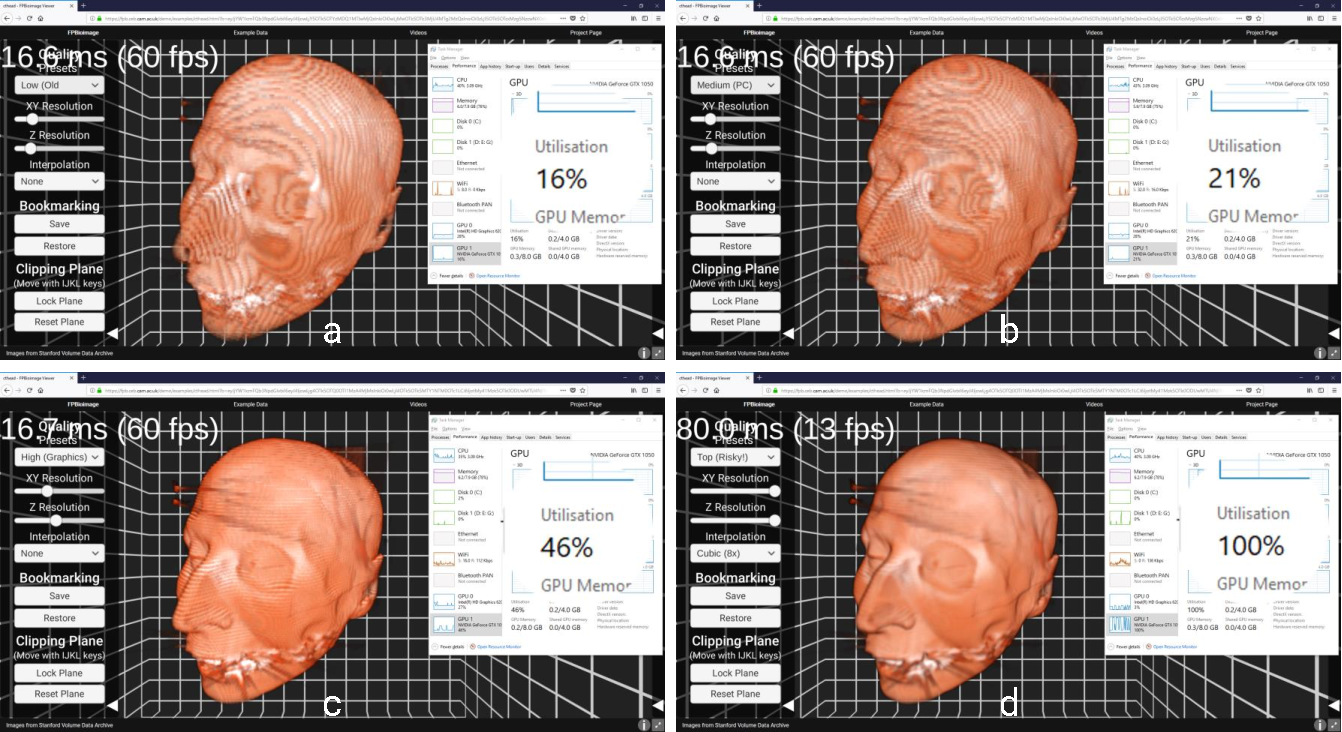
\includegraphics[width=\textwidth]{fpb-performance}
\caption[FPBioimage: Adjustable quality settings allow FPBioimage to be used on a range of devices]{The figure shows FPBioimage rendering with different quality presets: (a) Low; (b) Medium; (c) High; and (d) Top. The highest quality levels are designed for use on a high-end desktop computer; lower quality settings are provided to allow FPBioiamge to run on mobile devices. Performance was measured using frames per second (FPS) and graphics card percentage usage, shown on the screenshots. Results from these tests are presented in Table~\ref{tab:fpbPerformance}. The CT scan of a human head is from the Stanford Volumetric Data Archive~\cite{levoy1988volume}. }
\label{fig:fpb-quality}
\end{sidewaysfigure}

As XY-resolution is increased, performance decreases dramatically. 
This is because the number of pixels being rendered increases with the square of the XY-resolution number. 
It is interesting that XY-resolution does not have such a dramatic effect on the perceived visual quality, as shown in Figure~\ref{fig:fpb-quality}. 
Since there is little visual quality gain for a relatively large performance impact, XY-resolution is kept to moderate values even for the higher quality presets. 

Compared to the performance impact of XY-resolution, Z-resolution has a relatively small impact. 
From a Z-resolution of \SIrange{256}{768}{steps} the GPU use increases linearly. 
As shown in Figure~\ref{fig:fpb-quality}, however, Z-resolution has a considerable impact on visual quality of 3D images. 
For an equivalent impact on performance, an increase in Z-resolution gives better visual quality than an increase in XY-resolution; therefore providing high Z-resolution is prioritised for the presets. 

Interpolation of voxels has a big impact on visual quality, removing the staircase effect shown in Figure~\ref{fig:fpb-quality}, but also has a big impact on performance. 
When 2X interpolation is used, two voxels from the 2-nearest Z-planes to the marching ray's current position are averaged (weighted by distance) to smooth the appearance of the volume. 
This requires an extra texture lookup at every z-step for every screen pixel, causing a significant performance impact particularly at high XY- or Z-resolutions. 
In 8X interpolation, the 8-nearest voxels to the marching ray's position are used, requiring 8 texture lookups at every z-step. 
The extra texture lookups explains the high impact on performance of interpolation. 

The `Top' preset setting sets all quality variables to maximum, and the user is warned that this setting is `risky' because it can crash the web browser!
This is an impractical setting on most personal machines - Table~\ref{tab:fpbPerformance} shows that the GPU is working at full capacity, and only rendering \SI{9}{FPS}. 
However, on dedicated graphics workstations where the GPU is able to render \SI{60}{FPS} at top quality a fly-through video for publication can be recorded in real-time. 

\section{FPBioimage Suite}
FPBioimage is a volumetric renderer designed to be used in a web browser. 
However, to assist users uploading their 3D data to share on the internet, plugins are available for the open-source image analysis platforms ImageJ, FIJI, and Icy. 
Furthermore, thanks to its open-source nature and an easy-to-use JSON interface, other groups have been able to integrate FPBioimage into their own software packages, for example OMERO-FPBioimage. 
Finally, for users who want to view volumetric data on their mobile, I have created dedicated Android and iOS apps, which support virtual reality for truly immersive interaction with the data. % and Oculus?  
Together with FPBioimage, this collection of applications has been branded FPBioimage Suite.

\subsection{Plugins are available for popular image analysis programs}
After the initial release of FPBioimage~\cite{fantham2017new}, uploading data to share with others was a convoluted process. 
Users had to download a copy of FPBioimage, install it on their own personal web server, upload a stack of PNG files with a specific naming convention, edit some JavaScript on a template webpage, and finally share the web link. 
This is not an issue for any web developer, but was beyond the ability of many scientists who gather volumetric data. 
Whilst many users enjoyed viewing data with FPBioimage, very few used it to share their own data.

In order to simplify the upload process, I created the FPBioimage Helper plugin for the popular open-source image analysis programs ImageJ, FIJI, and Icy. 
These programs all support volumetric image data in a wide variety of formats thanks to OME Bioformats~\cite{linkert2010metadata}. 
Users simply have to open their 3D data in the program, click one button, and the plugin will output a web link that the researcher can share with others. 

By default, FPBioimage Helper will upload a simple webpage displaying the data to an Amazon Web Services (AWS) site.
If the user would prefer to host their data on a private web server, for example to implement password protection or use their own website template, they can choose not to upload the data but simply save the formatted images and website to their local machine for their own purpose. 

Using the plugin, rather than manually uploading PNG image slices, also provides faster download times for those viewing the data.
Instead of saving every plane as a separate PNG file, the plugin arranges images into texture atlases as described in Section~\ref{sec:fpbVolumeRendering}. 
A line of JSON (\texttt{'atlasMode': true}) tells FPBioimage to expect atlases, rather than individual image slices, reducing the number of downloads to 8. 
This reduces loading times in four ways: the overhead time associated with each download is reduced from number-of-slices to just 8; overall download size is smaller, because the PNG compression algorithm is able to exploit more informational redundancy~\cite[\textit{ch. 1}]{jayaraman2011digital}; the 8 texture atlases can be downloaded in parallel; and FPBioimage can skip the step of arranging slices into texture atlases, since it can send the downloaded atlases directly to the graphics card. 

The plugin is distributed as an ``update site'' through the FIJI updater, and also through the Icy online plugin repository. 
This makes it easy to keep up-to-date, so that users get the access to the latest features with as little effort as possible. 

\subsection{OMERO-FPBioimage integrates volume rendering with organised image repositories}
OMERO is a web-based platform for managing scientific images~\cite{moore2015omero}. 
Created by OME, the same team behind Bioformats, it integrates with a number of other software packages to help users upload their imaging data to a remote server, so that it can be accessed from anywhere. 
Furthermore a web interface makes it easy for OMERO users to share their data with others, allowing them to perform further analysis or even meta-studies on independent image sets~\cite{williams2017image}.

After reading about FPBioimage in \textit{Nature Photonics}, an OMERO user noticed that the two programs have similar goals, and suggested integrating FPBioimage into OMERO as the default volume renderer~\cite{ehrenfeuchter2017comment}. 
Thanks to FPBioimage's clear documentation and simple JSON interface, the OMERO team were able to incorporate an FPBioimage viewer into their software before any contact with me. 

\begin{figure}[htbp!]
\centering
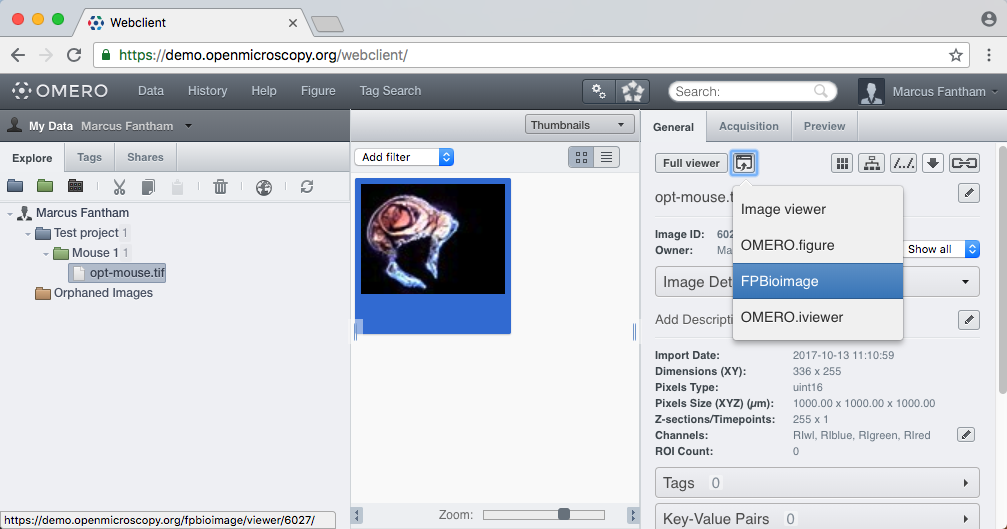
\includegraphics[width=1.0\textwidth]{fpb-omero}
\caption[FPBioimage: OMERO.web uses FPBioimage as its default renderer for 3D data]{The screenshot shows OMERO.web, which uses FPBioimage as its default volumetric image viewer. } % Will probably have two subfigures?
\label{fig:fpbOMERO}
\end{figure}

If a user opens a volumetric image in OMERO, an option appears in the viewer options to open in FPBioimage, as shown in Figure~\ref{fig:fpbOMERO}. 
When selecting this option, the OMERO server quickly creates a static webpage with an FPBioimage viewer and the relevant JSON to load the data into FPBioimage. 
Close collaboration with the OMERO team means that OMERO now sends texture atlases directly to FPBioimage, reducing loading time for users. 

The viewer has proved popular with OMERO users, finding diverse uses from plant sciences to pathology~\cite{fleur2018fpbioimage}.
It has been adopted as OMERO's default volumetric viewer, and is featured prominently on their webpage~\cite{omero2018website}.

\subsection{Mobile apps bring volume rendering to smartphones and virtual reality}
Since FPBioimage is a web-based application, it will run on any device with a web browser. 
This includes mobile devices, such as iPhones and Android smartphones, as well as tablet devices such as an iPad. 
However, mobile browsers have limited access to the device's computational resources, causing long loading times and poor performance, characterised by a low frame rate. 

To allow FPBioimage to run on mobiles with full performance, native apps were compiled for the Android and iOS operating systems, which are available through their respective app stores. 
Since mobiles usually only run one app at a time, the app has full access to all the computational and graphics processing capability of the device. 

For the mobile apps, a universal linking scheme has been devised. 
This means that if a user visits a website with an FPBioimage viewer on it, they will get the option to open the data in a native app on their phone instead of in the mobile browser. 
Since the mobile app uses the same rendering algorithm (presented in Section~\ref{sec:fpbVolumeRendering}) as the online app, the visualisation will be exactly the same. 

\begin{figure}[htbp!]
\centering
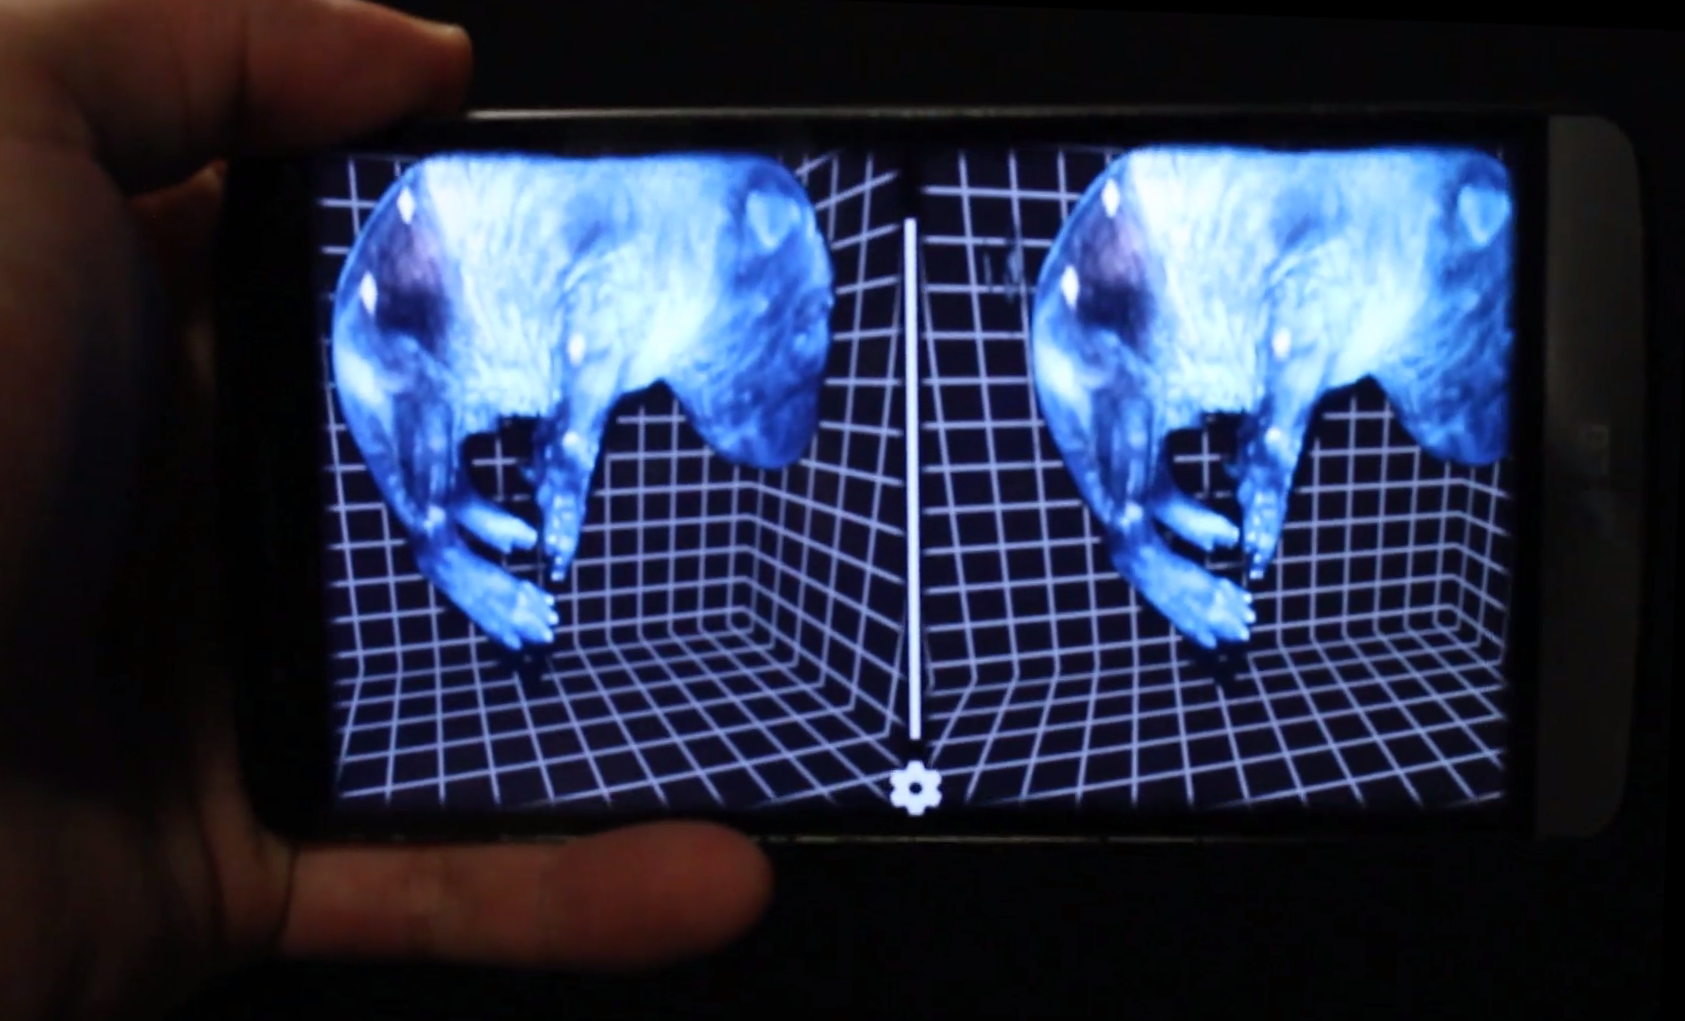
\includegraphics[width=1.0\textwidth]{fpb-android}
\caption[FPBioimage: The FPBioimage mobile app provides volumetric rendering in virtual reality]{FPBioimage has native apps for Android and iOS. The photo shows a split-screen stereo view, which can be used in conjunction with Google Cardboard\cite{cardboard} to support virtual reality. Data from~\cite{sharpe2002optical}. } % 
\label{fig:fpbMobile}
\end{figure}

As part of the port to mobile, a new focus was put on FPBioimage touch controls. 
Users can intuitively rotate the model by touching and dragging. 
Users can also zoom in and out by a two-finger pinch, and move around the model using two fingers and dragging. 
As with the web app, the quality can be changed to accommodate a range of mobile chipsets, and the usual rendering options of opacity, intensity and cutoff are available, along with the various projection methods.  

Running on mobile brings one more advantage, thanks to the low-cost virtual reality (VR) device Google Cardboard\cite{cardboard}. 
This is a VR viewer - originally made of cardboard but now available in more robust plastic models~\cite{get2018cardboard} - which utilises a smartphone's high-resolution screen and precise accelerometer to provide a low-cost VR experience. 
The user simply has to open their data in the mobile app, click the "Start VR" button, and put their phone into their Cardboard viewer. 
This option allows users to view their data in VR, providing a truly immersive experience and giving a perspective of the data not possible through any other means. 

%Oculus rift?? :( 


\section{Conclusion} % Replaces the `examples of use' section
As an online volumetric rendering program, FPBioimage has a wide range of uses which have not been possible before. 

As a volumetric renderer, FPBioimage offers a number of volumetric rendering modes found in most offline volume visualisation software, including composite ray marching and maximum intensity projections. 
However all other volume rendering programs have a complicated array of settings for changing transparency and colour maps, and no option for adjusting quality.
With a focus on ease-of-use from its conception, FPBioimage provides an interface that anyone can use, even non-expert users. 

Furthermore, because FPBioimage is designed to run on the web, or on devices with limited computational resources, the rendering algorithms have been optimised such that full-quality volume rendering can be performed in real time. 
This real-time performance has not been seen in other software. 
Indeed, the ease-of-use coupled with high performance have generated many requests that FPBioimage could be used as the default volumetric viewer in other image analysis software~\cite{twitter2018fantm}. 

In combination with the ImageJ, FIJI, or Icy plugins, scientists collecting volume data can share it with anyone in the world in one click. 
Data is uploaded to a public repository hosted on Amazon Web Services, at a permanent link, or can be uploaded to a private server for password protection. 
This allows researchers to get unprecedented instant feedback from international collaborators. 

\begin{figure}[htbp!]
\centering
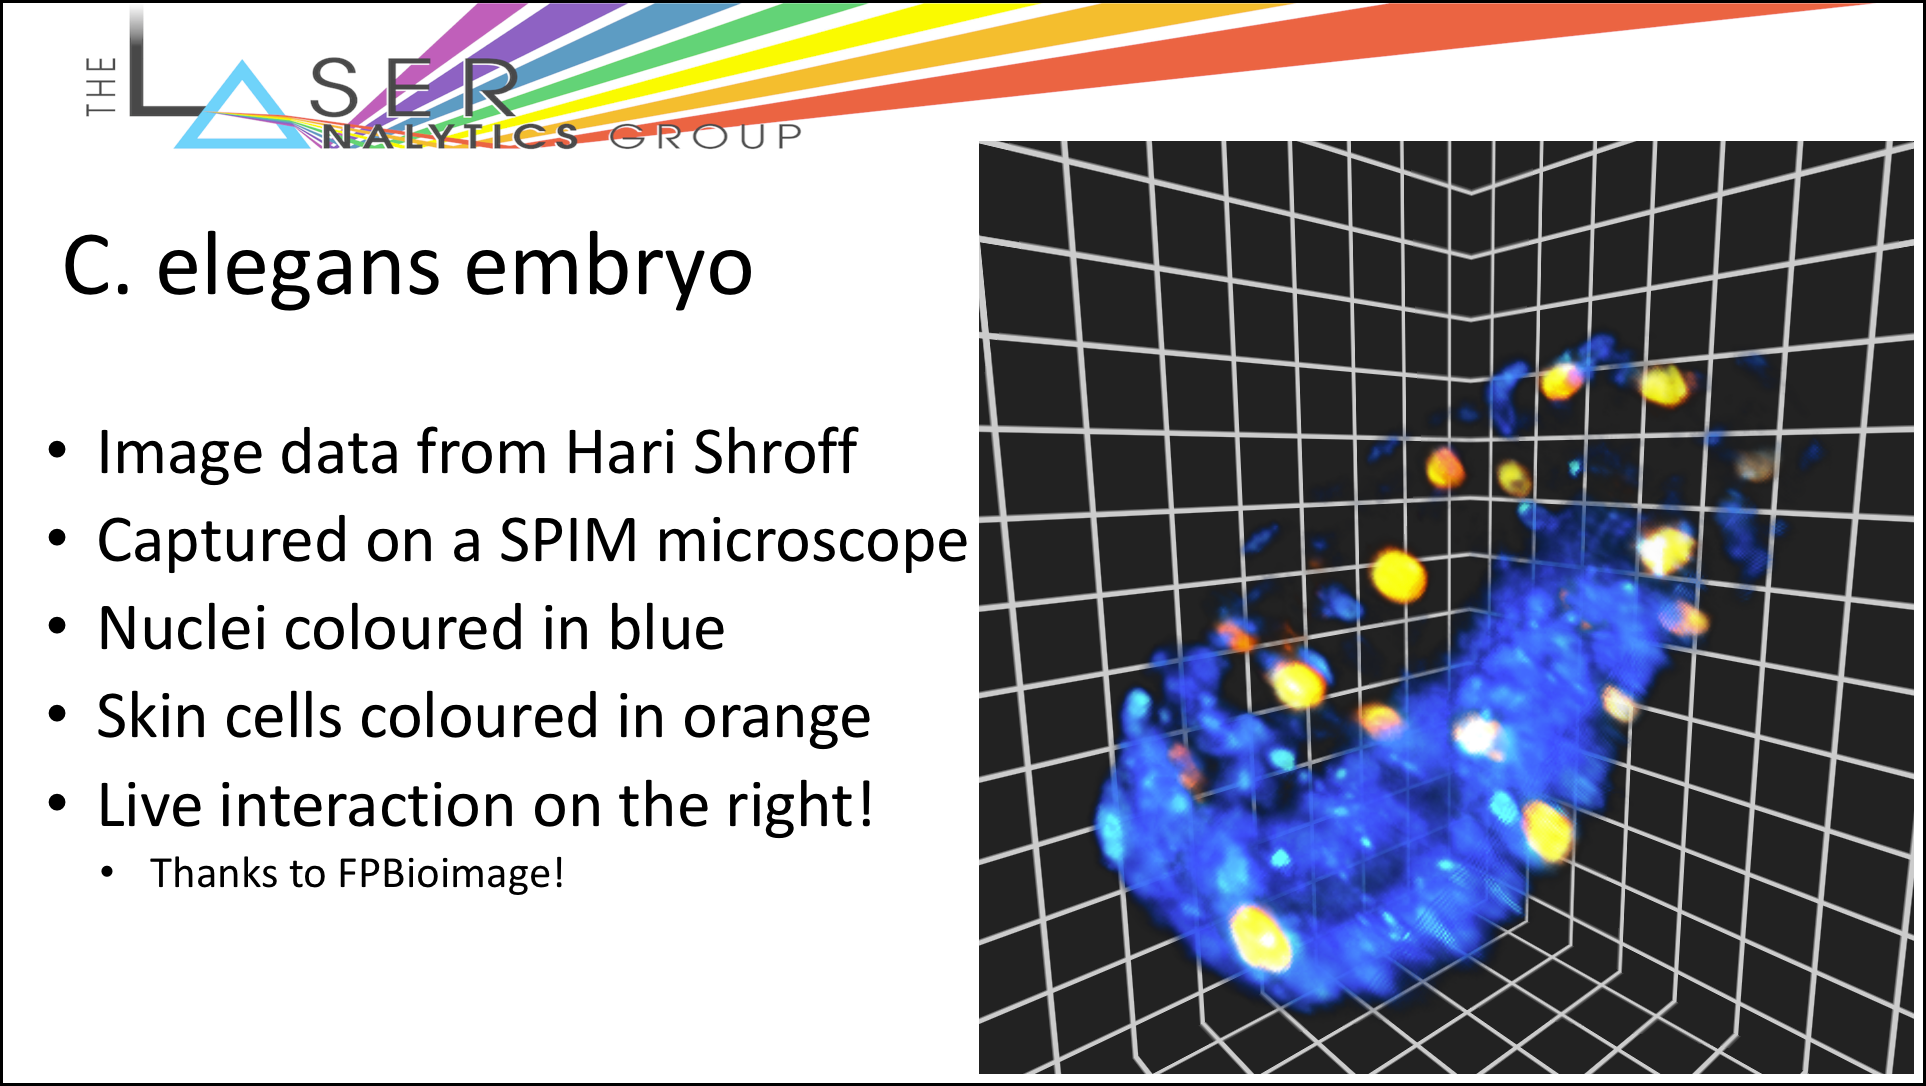
\includegraphics[width=1.0\textwidth]{fpb-liveslides}
\caption[FPBioimage: LiveSlides in Powerpoint brings interactive FPBioimage rendering to presentations]{Using the Powerpoint plugin LiveSlides, FPBioimage can be embedded in a presentation, bringing an interactive dynamic to explaining volumetric data. Data from~\cite{kumar2014dual}. } % 
\label{fig:fpb-liveslides}
\end{figure}

Researchers can embed FPBioimage in a presentation by utilising a slideshow plugin such as LiveSlides~\cite{liveslides}, as shown in Figure~\ref{fig:fpb-liveslides}. 
This allows an interactive flight through the data whilst talking about it, bringing a new dynamic to presentations and allowing detailed responses to questions which are not possible with a pre-recorded video. 

Finally, for sharing volumetric data with the wider community FPBioimage can be used as a publication tool. 
A whole set of 3D images can be uploaded, such that readers can explore for themselves the findings of an experiment~\cite{teplensky2017temperature}.
It is hoped that journals will adopt FPBioimage as a dynamic viewer for online publications, so that readers can interact with data alongside the text. 

FPBioimage makes sharing of volumetric data with anyone in the world a one-click operation, and introduces a new paradigm for publishing 3D image data. 